%%%%%%%%%%%%%%%%%%%%%%%%%%%%%%%%%%%%%%%%%%%%%%%%%%
%% Bachelor's & Master's Thesis Template        %%
%% Copyleft by Dawid Weiss & Marta Szachniuk    %%
%% Faculty of Computing and Telecommunication   %%
%% Poznan University of Technology, 2020        %%
%%%%%%%%%%%%%%%%%%%%%%%%%%%%%%%%%%%%%%%%%%%%%%%%%%


% Szkielet dla pracy licencjackiej pisanej w języku polskim.

\documentclass[polish,bachelor,a4paper,oneside]{ppfcmthesis}

\usepackage[utf8]{inputenc}
\usepackage[OT4]{fontenc}
\usepackage{longtable}
\usepackage[table,xcdraw]{xcolor}
\usepackage{float} 
\usepackage{hyperref}
\usepackage{listings}

%--------------------------------------
% Strona tytułowa
%--------------------------------------

\author{%
    Bartosz Adamczewski  \album{151764} \and
    Kacper Kuras \album{151783} \and
    Jakub Wieczorek \album{151888} \and
    Kacper Woźniak \album{151118} \and
}
\authortitle{}                                % Do not change.

\title{System do modelowania scenariuszy ćwiczeń radzenia sobie z sytuacjami kryzysowymi}

% Your supervisor comes here.
\ppsupervisor{dr inż. Sylwia Kopczyńska}

% Year of final submission (not graduation!)
\ppyear{2025}


\begin{document}

% Front matter starts here
    \frontmatter\pagestyle{empty}%
    \maketitle\cleardoublepage%


%--------------------------------------
% Spis treści
%--------------------------------------

    \pagenumbering{Roman}\pagestyle{ppfcmthesis}%
    \tableofcontents*
    \cleardoublepage % Zaczynamy od nieparzystej strony

%--------------------------------------
% Rozdziały
%--------------------------------------

%Najwygodniej jeśli każdy rozdział znajduje się w oddzielnym pliku
    \mainmatter%
    
\chapter{Wstęp}

Wstęp do pracy powinien zawierać następujące elementy:
\begin{itemize}
    \item krótkie uzasadnienie podjęcia tematu;
    \item cel pracy (patrz niżej);
    \item zakres (przedmiotowy, podmiotowy, czasowy) wyjaśniający, w jakim rozmiarze praca będzie realizowana;
    \item ewentualne hipotezy, które autor zamierza sprawdzić lub udowodnić;
    \item krótką charakterystykę źródeł, zwłaszcza literaturowych;
    \item układ pracy (patrz niżej), czyli zwięzłą charakterystykę zawartości poszczególnych rozdziałów;
    \item ewentualne uwagi dotyczące realizacji tematu pracy np.~trudności, które pojawiły się w trakcie
    realizacji poszczególnych zadań, uwagi dotyczące wykorzystywanego sprzętu, współpraca z firmami zewnętrznymi.
\end{itemize}

\noindent
\textbf{Wstęp do pracy musi się kończyć dwoma następującymi akapitami:}
\begin{quote}
    Celem pracy jest opracowanie / wykonanie analizy / zaprojektowanie / ...........
\end{quote}
oraz:
\begin{quote}
    Struktura pracy jest następująca. W rozdziale 2 przedstawiono przegląd literatury na temat ........
    Rozdział 3 jest poświęcony ....... (kilka zdań).
    Rozdział 4 zawiera ..... (kilka zdań) ............ itd.
    Rozdział X stanowi podsumowanie pracy.
\end{quote}

W przypadku prac inżynierskich zespołowych lub magisterskich 2-osobowych, po tych dwóch w/w akapitach
musi w pracy znaleźć się akapit, w którym będzie opisany udział w pracy poszczególnych członków zespołu. Na przykład:

\begin{quote}
    Jan Kowalski w ramach niniejszej pracy wykonał projekt tego i tego, opracował ......
    Grzegorz Brzęczyszczykiewicz wykonał ......, itd.
\end{quote}


    \chapter{Wymagania}

\section{Diagram kontekstu}
\begin{figure}[h!]
    \centering
    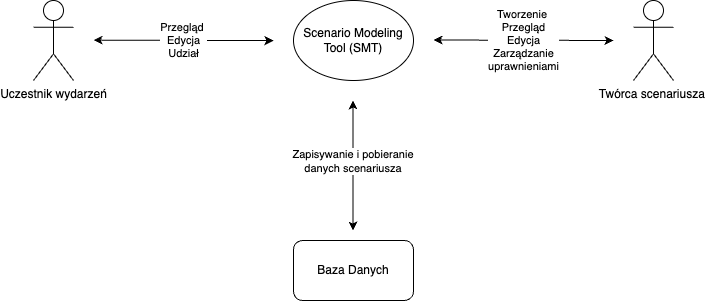
\includegraphics[width=0.99\textwidth]{resources/local/diagram-kontekstu.png}
    \caption{Diagram kontekstu}
\end{figure}

\section{Aktorzy}

\subsection{Twórca scenariusza}
Twórca scenariusza to osoba, która jest odpowiedzialna za tworzenie scenariuszy i ich modyfikowanie oraz dostosowywanie. 
Ma on możliwość definiowania wątków, obiektów, typów obiektów, szablonów, asocjacji, a także faz scenariusza w zależności 
od potrzeb i wymagań. Twórca scenariuszy może również nadawać uprawnienia edycji lub podglądu innym użytkownikom.

\subsection{Uczestnik wydarzeń}
Uczestnik wydarzeń to osoba biorąca udział w ćwiczeniach. Otrzymuje on dostęp do przeglądania lub modyfikacji scenariusza, 
w zależności od nadanych uprawnień. Dzięki temu podziałowi system jest odporny na wszelkie próby naruszenia integralności danych.

\section{Obiekty biznesowe}

\subsection{Scenariusz}
Scenariusz reprezentuje złożoną strukturę organizacyjną służącą do modelowania i symulacji sekwencji wydarzeń zachodzących 
w określonych ramach czasowych. Jest to centralny element systemu, który integruje i zarządza wieloma powiązanymi komponentami: 
wydarzeniami, wątkami, fazami i obiektami. Sam bezpośrednio zawiera metadane opisujące jego kontekst. 
Za jego pomocą zaimplementowany jest system uprawnień kontrolujący dostęp użytkowników.

\subsection{Faza scenariusza}
Faza scenariusza reprezentuje logiczny, wydzielony przedział czasowy w ramach całego scenariusza. 
Pozwala na podział scenariusza na mniejsze, znaczące etapy, ułatwiając organizację i wizualizację wydarzeń.

\subsection{Typ}

Typy służą do kategoryzacji i definiowania zasad zachowania elementów w systemie. Stanowią podstawę do zachowania spójności 
i prawidłowych relacji między elementami w systemie. Wyróżniamy dwa podstawowe rodzaje:
\begin{itemize}
    \item Typ Obiektu - jest to definicja kategorii obiektu występującego w scenariuszu. 
    Określa jego podstawowe cechy i zachowania, w tym konieczność globalnego dostępu do obiektu, 
    możliwość przypisania do niego użytkownika czy przynależność do szerszej kategorii (występuje hierarchia).
    \item Typ Asocjacji - Definiuje dozwolony rodzaj relacji między obiektami w systemie. 
    Określa typy obiektów które mogą wchodzić ze sobą w interakcje.
\end{itemize}

\subsection{Szablon}

Szablony definiują wzorce dla obiektów i ich atrybutów, umożliwiając standaryzację i automatyzację procesu tworzenia nowych 
elementów w scenariuszach.

\begin{itemize}
    \item Szablon Obiektu - Stanowi wzorzec definiujący strukturę i domyślne właściwości dla grupy podobnych obiektów. 
    Określa zarówno typ obiektu, do którego jest przypisany jak i wymagane atrybuty.
    \item Szablon Atrybutu - Definiuje pojedynczą cechę, którą mogą posiadać obiekty danego szablonu.
    Szablony pozwalają na szybkie i spójne tworzenie nowych elementów w systemie, zapewniając standardowy zestaw właściwości 
    i wartości początkowych.
\end{itemize}

\subsection{Obiekt}

Obiekt stanowi podstawową jednostkę w scenariuszu, reprezentującą konkretny element posiadający zdefiniowane atrybuty i 
mogący wchodzić w relacje z innymi obiektami. System rozróżnia obiekty globalne tworzone w wątku globalnym i dostępne w każdym 
innym oraz obiekty lokalne przypisane do konkretnych wątków i niedostępne w danym czasie w żadnym innym. 
Jedynym sposobem ich przekazania dalej są operacje rozgałęzień na wątkach.
Każdy obiekt tworzony jest na podstawie szablonu określającego jego strukturę.

\subsection{Asocjacja}

Asocjacje reprezentują relacje między obiektami w scenariuszu. Mogą być tworzone i usuwane w ramach wydarzeń.

\subsection{Atrybut}

Atrybuty definiują właściwości obiektów, które mogą zmieniać się w czasie trwania scenariusza. Każdy atrybut jest tworzony 
na podstawie szablonu obiektu określającego jego cechy domyślnie przyjmuje wartość zdefiniowaną w szablonie.

\subsection{Wątek}

Wątek reprezentuje sekwencję wydarzeń w scenariuszu, pozwalając na modelowanie równoległych ciągów wydarzeń. 
Trwają określoną liczbę akcji. W systemie występują dwa rodzaje wątków:
\begin{itemize}
    \item Wątek Globalny:
    \begin{itemize}
        \item Jest jeden na scenariusz,
        \item Zawiera wydarzenia globalne wpływające na wszystkie pozostałe wątki,
        \item Przechowuje obiekty globalne dostępne w całym scenariuszu.
    \end{itemize}
    \item Wątki Lokalne:
    \begin{itemize}
        \item Reprezentują niezależne sekwencje wydarzeń,
        \item Zawierają własne, lokalne obiekty,
        \item Mogą być łączone lub rozdzielane za pomocą rozgałęzień.
    \end{itemize}
\end{itemize}

\subsection{Rozgałęzienie}

Wątki mogą na siebie oddziaływać poprzez operacje:
\begin{itemize}
    \item FORK - podział jednego wątku na wiele, wraz z dystrybucją obiektów - definiowaną przez użytkownika.
    \item JOIN - łączenie wielu wątków w jeden, wraz z przekazaniem ich obiektów.
\end{itemize}

\subsection{Wydarzenie}

Wydarzenie trwa zawsze jedną akcję. Opisuje zachodzące w określonym momencie scenariusza zmiany (także te wpływające na organizację 
wątków). System rozróżnia następujące typy wydarzeń:
\begin{itemize}
    \item START/END - kontrolują rozpoczęcie i zakończenie wątku.
    \item NORMAL - standardowe wydarzenia w wątku lokalnym.
    \item GLOBAL - wydarzenia w wątku globalnym (najwyższy priorytet).
    \item FORK\_IN/FORK\_OUT - obsługują proces podziału wątku.
    \item JOIN\_IN/JOIN\_OUT - obsługują proces łączenia wątków.
    \item IDLE - wydarzenia puste, brak zmian w wątku.
\end{itemize}

Tylko wydarzenia IDLE, NORMAL oraz GLOBAL są bezpośrednio tworzone przez użytkownika. 
W wydarzeniach NORMAL oraz GLOBAL następują modyfikacje atrybutów obiektów oraz zarządzanie asocjacjami między nimi.

\newpage
\section{Diagram przypadków użycia}
\begin{figure}[h!]
    \centering
    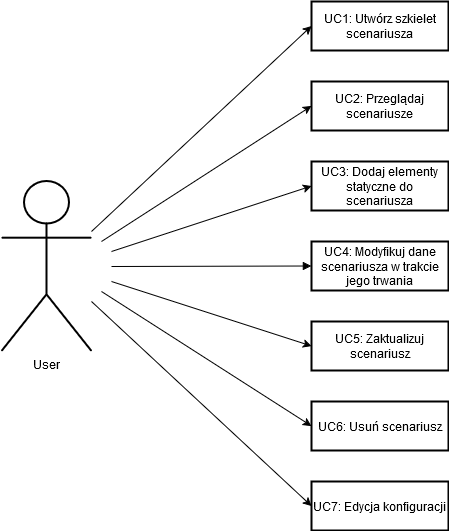
\includegraphics[width=0.5\textwidth]{resources/local/use-case-diagram-2.png}
    \caption{Diagram przypadków użycia}
    \label{fig:use_case_diagram}
\end{figure}

\section{Tabela przypadków użycia}
\small{
\begin{longtable}{|p{1cm}|p{4.5cm}|p{8cm}|}
    \hline
    \textbf{ID} & \textbf{Przypadek użycia} & \textbf{Opis} \\
    \hline
    \endfirsthead
    \caption[]{Tabela przypadków użycia -- ciąg dalszy} \\
    \hline
    \textbf{ID} & \textbf{Przypadek użycia} & \textbf{Opis} \\
    \hline
    \endhead
    \hline
    \endfoot
    \hline
    \caption{Tabela przypadków użycia} \label{tab:use_case_table} \\
    \endlastfoot
    UC1 & Utwórz szkielet scenariusza & Użytkownik tworzy scenariusz podając jego czas wraz z pozostałymi właściwościami go opisującymi. System dodaje nowy scenariusz wraz z domyślnymi danymi tworzonymi dla nowego scenariusza. \\
    \hline
    UC2 & Przeglądaj scenariusze & Użytkownik przegląda listę dostępnych scenariuszy, z opcją filtrowania, która umożliwia wybranie konkretnego scenariusza oraz jego edycję lub usunięcie. \\
    \hline
    UC3.1 & Utwórz szablon obiektu & Użytkownik tworzy szablon obiektu dostępny we wszystkich scenariuszach. \\
    \hline
    UC3.2 & Utwórz obiekt & Użytkownik tworzy konkretny obiekt przypisany do scenariusza. \\
    \hline
    UC3.3 & Utwórz szablon atrybutu & Użytkownik tworzy szablon atrybutu przyporządkowany do danego szablonu obiektu. \\
    \hline
    UC3.4 & Utwórz typ obiektu & Użytkownik tworzy typ obiektu dostępny we wszystkich scenariuszach. \\
    \hline
    UC3.5 & Utwórz typ asocjacji & Użytkownik tworzy typ asocjacji dostępny we wszystkich scenariuszach. \\
    \hline
    UC3.6 & Utwórz asocjację & Użytkownik tworzy asocjację pomiędzy dwoma obiektami z danego scenariusza. \\
    \hline
    UC4.1 & Utwórz wątek & Użytkownik tworzy nowy wątek poprzez rozdzielenie wątku istniejącego lub dodanie nowego osobnego wątku. \\
    \hline
    UC4.2 & Utwórz zdarzenie & Użytkownik tworzy zdarzenie wraz ze zdefiniowaniem zmian w asocjacjach lub atrybutach obiektów. \\
    \hline
    UC5.1 & Edycja danych podanych przy tworzeniu scenariusza & Użytkownik modyfikuje właściwości scenariusza podane podczas jego tworzenia. \\
    \hline
    UC5.2 & Edycja elementów statycznych oraz zdarzeń & Użytkownik modyfikuje istniejące elementy statyczne (np. obiekty, atrybuty) wraz z właściwościami zdarzeń i wątków. \\
    \hline
    UC.6.1 & Usuń scenariusz & Użytkownik usuwa scenariusz po jego wybraniu z listy. System pyta o potwierdzenie i usuwa scenariusz wraz z danymi prywatnymi dla scenariusza na stałe. \\
    \hline
    UC.6.2 & Usuń element statyczny & Użytkownik posiada opcję usunięcia: typu asocjacji oraz obiektu, szablonu obiektu oraz atrybutu, konkretnego obiektu, wątku, rozgałęzienia i fazy.    \\
    \hline
    UC.7 & Edycja konfiguracji & Użytkownik edytuje konfigurację. System wykorzystuje zdefiniowane właściwości przy tworzeniu nowego scenariusza. \\
    \hline
\end{longtable}
}
\normalsize
\section{Wymagania pozafunkcjonalne}
Wymagania pozafunkcjonalne są zgodne ze standardem ISO 25010, zdefiniowanym w książce 
\emph{Systems and Software Engineering — Systems and Software Quality Requirements and Evaluation (SQuaRE) — System and Software Quality Models} 
\cite{iso25010} i zostały opisane w poniższej tabeli:

\section{Tabela wymagań pozafunkcjonalnych}
\small{
\begin{longtable}{|p{1cm}|p{2.5cm}|p{4.5cm}|p{5cm}|}
    \hline
    \textbf{ID} & \textbf{ISO 25010} & \textbf{Wymaganie} & \textbf{Realizacja} \\
    \hline
    \endfirsthead
    \caption[]{Tabela wymagań pozafunkcjonalnych -- ciąg dalszy} \\
    \hline
    \textbf{ID} & \textbf{ISO 25010} & \textbf{Wymaganie} & \textbf{Realizacja} \\
    \hline
    \endhead
    \hline
    \endfoot
    \hline
    \caption{Tabela wymagań pozafunkcjonalnych} \label{tab:NFR-table} \\
    \endlastfoot
    NFR1 & Funkcjonalność & System powinien dostarczać wszystkie wymagane funkcje. & Implementacja zgodnie z przedstawionymi wymaganiami.\\
    \hline
    NFR2 & Funkcjonalność & Funkcje systemowe powinny działać zgodnie z wymaganiami dostarczając odpowiednie odpowiedzi. & Sprawdzenie przy pomocy testów integracyjnych i jednostkowych. \\
    \hline
    NFR3 & Wydajność & Aplikacja powinna umożliwiać efektywne zarządzanie żądaniami. &  Osiągnięte dzięki optymalizacji transakcji i dostępu do bazy danych poprzez wykorzystanie mechanizmu keylock w celu unikania konfliktów podczas równoczesnego dostępu do danych. \\
    \hline
    NFR4 & Wydajność & System musi spełniać wymóg skalowalności w celu obsługi wielu użytkowników bez znaczącego spadku wydajności. & Realizacja poprzez zastosowanie mikroserwisową architekturę. \\
    \hline
    NFR5 & Zgodność & System powinien współpracować z innymi systemami. & Osiągnięte dzięki wykorzystaniu websocketa oraz integracji za pomocą REST API. \\
    \hline
    NFR6 & Zgodność & System powinien działać na różnych urządzeniach. & Zapewnienie responsywności poprzez implementację za pomocą CSS Media Queries. \\
    \hline
    NFR7 & Użyteczność & Aplikacja powinna zapewniać rozpoznawalność zastosowania. & Umożliwiło to zastosowanie czytelnego układu oraz zgodności z UX. \\
    \hline
    NFR8 & Użyteczność & System powinien zawierać czytelny i intuicyjny interfejs. & Realizacja przy użyciu frameworka React oraz komponentów w standardzie WCAG 2.1. \\
    \hline
    NFR9 & Użyteczność & System powinien odpowiednio stosować semantykę HTML. & Wykorzystanie odpowiednich znaczników HTML oraz frameworków, które wspierają A11y. \\
    \hline
    NFR10 & Użyteczność & Użytkownik powinien mieć pełną kontrolę za pomocą klawiatury. & Przeprowadzenie testów wszystkich komponentów aplikacji przy pomocy klawiatury. \\
    \hline
    NFR11 & Niezawodność & Aplikacja powinna radzić sobie z błędami. & Aplikacja zawiera system obsługi wyjątków oraz testy end to end. \\
    \hline
    NFR12 & Niezawodność & Kod aplikacji powinien zapewniać transakcyjność oraz integralność danych. & Wykorzystanie PostgreSQL, który umożliwia kontrolę integralności oraz operacja transakcyjne. \\
    \hline
    NFR13 & Łatwość utrzymania & System powinien spełniać zasady SOLID oraz modularność. & Uzyskanie poprzez implementację według zasad SOLID, co umożliwia łatwe dodawanie nowych funkcji. \\
    \hline
    NFR14 & Łatwość utrzymania & Zmiany logiki w warstwie nie powinny wymagać zmian w pozostałych warstwach. &  Zastosowanie odpowiedniej architektury wartstowej. \\
    \hline
    NFR15 & Łatwość utrzymania & System powinien być przystosowany do automatycznego testowania. & Wykorzystanie testów jednostkowych oraz testów end-to-end. \\
    \hline
    NFR16 & Bezpieczeństwo & Aplikacja powinna zawierać odpowiednie mechanizmy uwierzytelniania i autoryzacji. & Implementacja mechnizmów JWT oraz uprawienia użytkowników na podstawie ich ról. \\
    \hline
    NFR17 & Bezpieczeństwo & System powinien zwracać logi. & Dodanie kodów błędów na poziomie API Exception. \\
    \hline
    NFR18 & Przenośność  & System powinien być łatwy do wdrożenia w różnych środowiskach. & Wykorzystanie Dockera i Docker Compose.\\
    \hline
    NFR19 & Przenośność & Aplikacja powinna łatwa do uruchomienia. & Zastosowanie konteneryzacji oraz gotwych skryptów. \\
    \hline
\end{longtable}
}
\normalsize
    \chapter{Architektura}

\section{Markitektura 4+1}

\subsection{Diagram architektury}

\begin{figure}[h!]
    \centering
    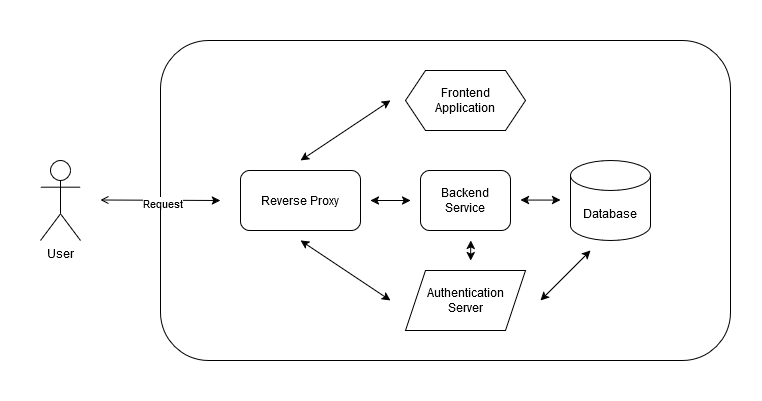
\includegraphics[width=0.99\textwidth]{resources/local/diagram-architektury.png}
    \caption{Diagram architektury}
\end{figure}

\subsection{Perspektywa logiczna}

\subsubsection*{Scenario manager}
Moduł globalny jest centralnym elementem systemu, odpowiedzialnym za zarządzanie scenariuszami użytkownika. \\

\textbf{Główne funkcje:}
\begin{itemize}
    \item Punkt wejściowy do widoku szczegółowego.
    \item Przedstawienie oraz umożliwienie zarządzania scenariuszami użytkownika.
\end{itemize}

\textbf{Kluczowe elementy:}
\begin{table}[H]
    \centering
    \begin{tabular}{|l|p{10cm}|}
        \hline
        \textbf{Element} & \textbf{Opis} \\
        \hline
        Lista scenariuszy & Zawiera scenariusze, do których użytkownik posiada uprawnienia. \\
        \hline
    \end{tabular}
\end{table}

\vspace{1em}

\subsubsection*{Object catalogue}
Moduł przeznaczony dla typów asocjacji oraz szablonów i typów obiektów.

\textbf{Główne funkcje:}
\begin{itemize}
    \item Przedstawienie oraz umożliwienie zarządzania danymi globalnymi.
\end{itemize}

\textbf{Kluczowe elementy:}
\begin{table}[H]
    \centering
    \begin{tabular}{|l|p{10cm}|}
        \hline
        \textbf{Element} & \textbf{Opis} \\
        \hline
        Lista szablonów obiektów & Przechowuje informacje o wszystkich szablonach obiektów. \\
        \hline
        Lista typów obiektów & Przechowuje informacje o wszystkich typach obiektów. \\
        \hline
        Lista typów asocjacji & Przechowuje informacje o wszystkich typach asocjacji. \\
        \hline
    \end{tabular}
\end{table}

\vspace{1em}

\subsubsection*{Timeline}
Moduł przeznaczony do wizualizacji scenariusza.

\textbf{Główne funkcje:}
\begin{itemize}
    \item Ukazanie faz oraz wątków scenariusza w czasie.
    \item Ukazanie zmian obiektów w poszczególnych momentach.
\end{itemize}

\textbf{Kluczowe elementy:}
\begin{table}[H]
    \centering
    \begin{tabular}{|l|p{10cm}|}
        \hline
        \textbf{Element} & \textbf{Opis} \\
        \hline
        Oś czasu & Ukazuje relacje pomiędzy wątkami oraz fazy scenariusza. \\
        \hline
        Widok szczegółowy wydarzenia & Ukazuje zmiany asocjacji oraz atrybutów obiektów. \\
        \hline
    \end{tabular}
\end{table}

\subsection{Perspektywa procesu}

Proces wysłania żądania przez istniejącego użytkownika systemu:

\textbf{Krok 1:} Klient wysyła żądanie HTTP/HTTPS do bramy wejściowej systemu, którą jest Reverse proxy. 

\textbf{Krok 2:} Reverse Proxy przekazuje żądanie do Authentication Server. 

\textbf{Krok 3:} Jeżeli dane autoryzacji są poprawne generowany oraz zwracany jest token JWT służący do autoryzacji. 

\textbf{Krok 4:} Wykonywane jest żądanie na konkretny endpoint Backend Service, wraz z wcześniej uzyskanym tokenem.

\textbf{Krok 5:} Żądanie jest realizowane poprzez kolejne warstwy aplikacji, skuktując zwróceniem statusu sukcesu lub błędu. 
W scenariuszu sukcesu, aplikacja najpewniej zrealizowała zmiany w Database lub zwróciła z niej dane.


\subsection{Perspektywa fizyczna}

System aktualnie nie funkcjonuje na żadnej infrastrukturze fizycznej lub chmurowej. Aczkolwiek, komponenty oraz ich zależności
zdefiniowane są za pomocą dockera, co w prosty sposób umożliwia uruchomienie systemu na środowisku produkcyjny lub w środowisku
deweloperskim (lokalnym), używanego w celu dalszego rozwoju projektu.

\subsection{Perspektywa implementacyjna}

\begin{itemize} 
    \item \textbf{Reverse Proxy} - Serwer proxy, jest bramą do systemu, która obsługuje ruch przychodzący i kieruje żądania HTTP/HTTPS do odpowiednich usług. W naszej architekturze rolę tę pełni \textbf{NGINX}.
    \item \textbf{Frontend Application} - Aplikacja webowa udostępniająca graficzny interfejs użytkownika (UI), stworzona przy użyciu frameworka React i języka TypeScript. Serwuje statyczne pliki (HTML, CSS, JS) i komunikuje się z backendem za pomocą API.
    \item \textbf{Backend Service} - Aplikacja stworzona za pomocą frameworka \textbf{Spring Boot} oraz języka Java, realizująca logikę biznesową, poprzez odpowiednie przetwarzanie żądań API oraz komunikację z bazą danych i serwerem uwierzytelniania.
    \item \textbf{Authentication Server} - Serwer uwierzytelniania i autoryzacji \textbf{Keycloak}. To popularne narzędzie umożliwia zarządzanie tożsamościami użytkowników zgodne z najnowszyszymi standardami.
    \item \textbf{Database} - Relacyjna baza danych \textbf{PostgreSQL}, przechowująca dane aplikacji.
\end{itemize}

\section{Decyzje architektoniczne}

\begin{table}[H]
    \centering
    \begin{tabular}{|p{4cm}|p{10cm}|}
        \hline
        \textbf{Decyzja} & \textbf{Opis} \\
        \hline
        Architektura klient-serwer & Jest to odpowiedni wybór dla naszych wymagań, ponieważ architektura ta 
        zakłada jasny podział ról: frontend (klient), backend (serwer), jest prosta do skalowania oraz umożliwia centralizację danych.  \\
        \hline
        Obsługa zapytań poprzez REST API & REST to najpopularniejsze rozwiązanie w architekturze klient-serwer. Bardzo dobrze pasuje
        do realizowania operacji CRUD, na ktorych opiera się nasza aplikacja. Integruje się także w prosty sposób z innymi usługami. \\
        \hline
        Websocket & Został użyty do dezauktualizowania danych, które zostały zmienione przez innego użytkownika. Umożliwia natychmiastowe
        powiadomienie frontendu o zajściu zmian w aktualnie wyświetlanym scenariuszu, poprzez analizowanie zmian w bazie danych. \\
        \hline 
        Użycie konteneryzacji &  Umożliwiło to nam uruchomienie wszystkich wymaganych komponentów systemu lokalnie w celu rozwoju aplikacji,
        oraz testowania jej działania. Konteneryzacja za pomocą Dockera ułatwi także firmie, która będzie kontynuowała projekt, dalszy
        rozwój aplikacji oraz ewentualnie uruchomienie serwisu na infrastrukturze fizycznej lub chmurowej. \\
        \hline
        Reverse Proxy jako punkt wejściowy systemu & 
        \begin{itemize}
            \setlength\itemsep{0.1em} 
            \item \textbf{Bezpieczeństwo:} ukrycie wewnętrznej struktury systemu oraz blokowanie podejrzanych adresów IP i ataków DDoS.
            \item \textbf{Wydajność:} równoważenie obciążenia oraz caching.
            \item \textbf{Skalowalność:} ułatwia wdrażanie systemu na etap produkcyjny.
        \end{itemize} \\
        \hline
        Keycloak zamiast własnego rozwiązania & Pozwoliło nam to na wprowadzenie mechanizmu 
        uwierzytelniania oraz autoryzacji zgodnego z najnoszymi standardami przy małym nakładzie czasu. System ten jest bardzo 
        elastyczny oraz skalowalny co ułatwi dalszy rozwój aplikacji. Udostępnia także użyteczny panel administartora, który w dostępny sposób
        umożliwia zarządzanie użytkownikami oraz konfiguracją. \\
        \hline
        Relacyjna baza danych & Dane w naszym systemie są strukturalne i wymagają relacji. Poszczególne obiekty w bazie danych wymagają
        jasno zdefiniowanych atrybutów. Wymagana jest także transakcyjność, dzięki czemu operacje są niezawodne, spójne oraz odtwarzalne.  \\
        \hline
    \end{tabular}
    \caption{Podjęte decyzje architektoniczne}
\end{table}

\section{Wykorzystane technologie}
W naszym projekcie wykorzystaliśmy następujące technologie:
\begin{description}
    \item[Java 21] Jest to obiektowy, wydajny i uniwersalny język programowania. Wybrany przez nas ze względu na to, że każdy z nas ma w nim doświadczenie, jest to jeden z najpopularniejszych języków programowania, posiada rozbudowane zaplecze bibliotek, a także jest łatwy w implementacji.
    \item[Spring Boot] Jest to framework używany do implementacji mechanizmów REST API, zawiera wiele bibliotek, które ułatwiają pracę nad projektem. Został przez nas wybrany ze względu na bardzo dobre działanie z językiem programowania Java 21.
    \item[PostgreSQL] Jest to system, który został stworzony w celu utrzymywania relacyjnych baz danych. Wybraliśmy go ze względu na wysoką wydajność, oraz dobrą integrację z naszym projektem.
    \item[Docker Compose] Używany przez nas w celu konteneryzacji, co zapewnia łatwe wdrożenie i odpalanie aplikacji w różnych środowiskach.
    \item[Nginx] Jest to oprogramownie działające jako serwer proxy.
    \item[TypeScript] Język programownia używany na frontendzie. Wybrany ze względu na łatwość implementacji oraz kontroli nad komponentami.
    \item[HTML i CSS] Podstawowe języki umożliwiające tworzenie struktury oraz stylizację aplikacji.
    \item[React] Jest to biblitoka, dostarczająca dynamiczne rozwiązania na frontendzie, łatwe tworzenie komponentów oraz dobrą integrację z API.
    \item[JUnit] Biblioteka używana do implementacji testów jednostkowych. Wybrana ze względu na perfekcyjną kompatybilność z Java 21.
    \item[Git] System kontrolii wersji oprogramowania. Zapewnia wysoką wydajność pracy zespołu.
    \item[Github] Platforma, która umożliwia zdalne utrzymywanie repozytorium projektu.
    \item[Github Issues] Używane jako miejsce, w którym zespół przypisywał oraz dzielił się zadaniami podczas sprintów.
    \item[Swagger] Narzędzie umożliwiające tworzenie dokumentacji API. Wybrane ze względu na kompatybilność z wcześniejszymi technologiami takimi jak Java 21 oraz Spring Boot oraz przez doświadczenie zespołu w tej technologii.
    \item[Postman] Oprogramowanie do testowania interfejsu API. Używana do bieżącego sprawdzania poprawności danych zapytań.
    \item[Husky] Narzędzie, które umożliwia lintowanie kodu lub sprawdzanie poprawności kodu przed commitem.
    \item[Intellij IDEA] Jest to środowisko programistyczne stworzone w celu tworzenia aplikacji w języku Java. Wybrane przez nas głównie ze względu na wszechstronność.
\end{description}

\section{Logika biznesowa}

\subsection{Dodawanie scenariusza}

\subsubsection{Cel operacji}
Utworzenie nowego scenariusza, który służy jako główny kontener organizujący wydarzenia, wątki i obiekty w określonych ramach czasowych.

\subsubsection{Operacja}
Proces dodawania scenariusza obejmuje:
\begin{enumerate}
    \item \textbf{Konfigurację podstawową}
    \begin{itemize}
        \item Określenie ram czasowych (data początku i końca).
        \item Zdefiniowanie jednostki czasu dla wydarzeń.
        \item Ustalenie metadanych (tytuł, opis, kontekst, cel).
    \end{itemize}
    \item \textbf{Inicjalizację struktury}
    \begin{itemize}
        \item Utworzenie wątku globalnego do zarządzania głównymi wydarzeniami.
        \item Przygotowanie dostępnych typów obiektów w scenariuszu.
    \end{itemize}
    \item \textbf{Konfigurację uprawnień}
    \begin{itemize}
        \item Przypisanie twórcy jako właściciela scenariusza.
        \item Nadanie pełnych uprawnień administracyjnych.
    \end{itemize}
\end{enumerate}

\subsubsection{Ograniczenia biznesowe}
\begin{itemize}
    \item Ramy czasowe muszą być logicznie spójne (data końcowa później niż początkowa).
    \item Każdy scenariusz musi mieć dokładnie jednego właściciela.
    \item Scenariusz musi posiadać wątek globalny do synchronizacji wydarzeń.
\end{itemize}

\subsubsection{Rezultat}
Utworzony scenariusz wraz z możliwymi do wykorzystania podstawowymi typami i zdefiniowanym wątkiem globalnym.

\subsection{Usuwanie scenariusza}

\subsubsection{Cel}
Usunięcie scenariusza wraz z zawartymi w nim wydarzeniami, wątkami i obiektami.

\subsubsection{Operacja}
Proces usuwania scenariusza obejmuje:
\begin{enumerate}
    \item \textbf{Usuwanie obiektów}
    \begin{itemize}
        \item Wraz z nimi usuwane są wszelkie ich zmiany.
    \end{itemize}
    \item \textbf{Usuwanie wątków}
    \begin{itemize}
        \item Usuwanie rozgałęzień.
        \item Usuwanie wydarzeń.
    \end{itemize}
    \item \textbf{Usuwanie samego scenariusza}
    \begin{itemize}
        \item Wraz z nim pozostałych powiązań.
    \end{itemize}
\end{enumerate}

\subsubsection{Ograniczenia biznesowe}
Usuwający musi być autorem scenariusza.

\subsubsection{Rezultat}
Usunięty scenariusz wraz z wszystkimi śladami jego obecności.

\subsection{Aktualizacja metadanych scenariusza}

\subsubsection{Cel}
Zmiana kontekstu scenariusza.

\subsubsection{Operacja}
Proces zmiany kontekstu scenariusza obejmuje wprowadzenie i zapisanie zmienionych informacji.

\subsubsection{Ograniczenia biznesowe}
Wprowadzone dane muszą istnieć (nie można wprowadzić wartości \texttt{null}).

\subsubsection{Rezultat}
Zmienione metadane scenariusza.

\subsection{Dodawanie wątku}

\subsubsection{Cel}
Dodanie nowego wątku w scenariuszu.

\subsubsection{Operacja}
Wątek może być dodany na dwa różne sposoby (nie uwzględniając wątku globalnego wstawianego automatycznie wraz z tworzeniem scenariusza). Istnieją trzy podstawowe sposoby dodania wątku - jeden bezpośredni i dwa pośrednie. 
Sposób bezpośredni obejmuje zwykłe wstawienie wątku w określonym czasie, natomiast pośrednie wstawienie rozgałęzień.
\begin{itemize}
    \item W przypadku "zwykłego" wątku obiekty możliwe są do dodania ręcznie.
    \item W przypadku łączenia wątków (\texttt{JOIN}) wszystkie obiekty z wątków wchodzących przekazywane są do nowego wątku.
    \item W przypadku podziału wątku należy zdefiniować, które obiekty mają być przekazane do którego potomka.
\end{itemize}

\paragraph{Bezpośredni} Proces wstawienia takiego wątku obejmuje:
\begin{enumerate}
    \item \textbf{Konfigurację podstawową}
    \begin{itemize}
        \item Zdefiniowanie podstawowych danych oraz czasu powstania wątku (konkretna akcja).
    \end{itemize}
    \item \textbf{Inicjalizację odpowiednich struktur}
    \begin{itemize}
        \item Dodanie wątku skutkuje wstawieniem wydarzeń \texttt{START} na jego początek oraz \texttt{END} na bezpośrednio kolejną akcję.
    \end{itemize}
\end{enumerate}

\paragraph{Pośredni}
Dodanie rozgałęzienia \texttt{JOIN} skutkuje utworzeniem jednego nowego wątku z połączenia innych, a \texttt{FORK} stworzeniem wielu wątków z jednego.

\subsubsection{Ograniczenia biznesowe}
W przypadku dodawania wątku bezpośrednio brak, dla rozgałęzień opisany oddzielnie.

\subsubsection{Rezultat}
Utworzenie nowego wątku.

\subsection{Zmiana informacji wątku}

\subsubsection{Cel}
Zmiana informacji określonych w wątku.

\subsubsection{Operacja}
Operacja obejmuje wprowadzenie zmienionych danych i ich zapisanie.

\subsubsection{Ograniczenia biznesowe}
Nie można wstawić pustych danych.

\subsubsection{Rezultat}
Zmiana danych wątku.

\subsection{Usuwanie wątku}

\subsubsection{Cel}
Usunięcie danego wątku.

\subsubsection{Operacja}
Ze względu na możliwe powiązania z innymi wątkami jest to operacja dość niebezpieczna, gdyż usuwa także wszystkie wątki bezpośrednio wynikające z usuwanego. 
\begin{enumerate}
    \item \textbf{Analizę wątków}
    \begin{itemize}
        \item Znajdowane są wszystkie wątki bezpośrednio wynikające z danego wątku za pomocą rozgałęzień.
        \item \texttt{FORK} w całości zależy od konkretnego wątku.
        \item \texttt{JOIN} tylko jeżeli wszystkie wątki wchodzące do niego zależą od jednego wątku.
        \item W przypadku pozostawienia jednego wątku wchodzącego do łączenia nie jest ono potrzebne i w dalszej części będzie usunięte.
    \end{itemize}
    \item \textbf{Usunięcie danych wątków}
    \begin{itemize}
        \item Usuwany jest dany wątek i wszystkie z niego wynikające.
        \item Usuwane są niepotrzebne rozgałęzienia.
    \end{itemize}
    \item \textbf{Usunięcie łączeń jeden-do-jednego}
    \begin{itemize}
        \item Wszystkie znalezione rozgałęzienia są usuwane.
        \item Wydarzenia wątku wychodzącego są przenoszone do wątku wchodzącego, który jest odpowiednio wydłużany.
    \end{itemize}
\end{enumerate}

\subsubsection{Ograniczenia biznesowe}
Brak.

\subsubsection{Rezultat}
Usunięcie wątku wraz z wszystkimi innymi, które były od niego zależne.

\newpage
\section{Schemat bazy danych}

\begin{figure}[h!]
    \centering
    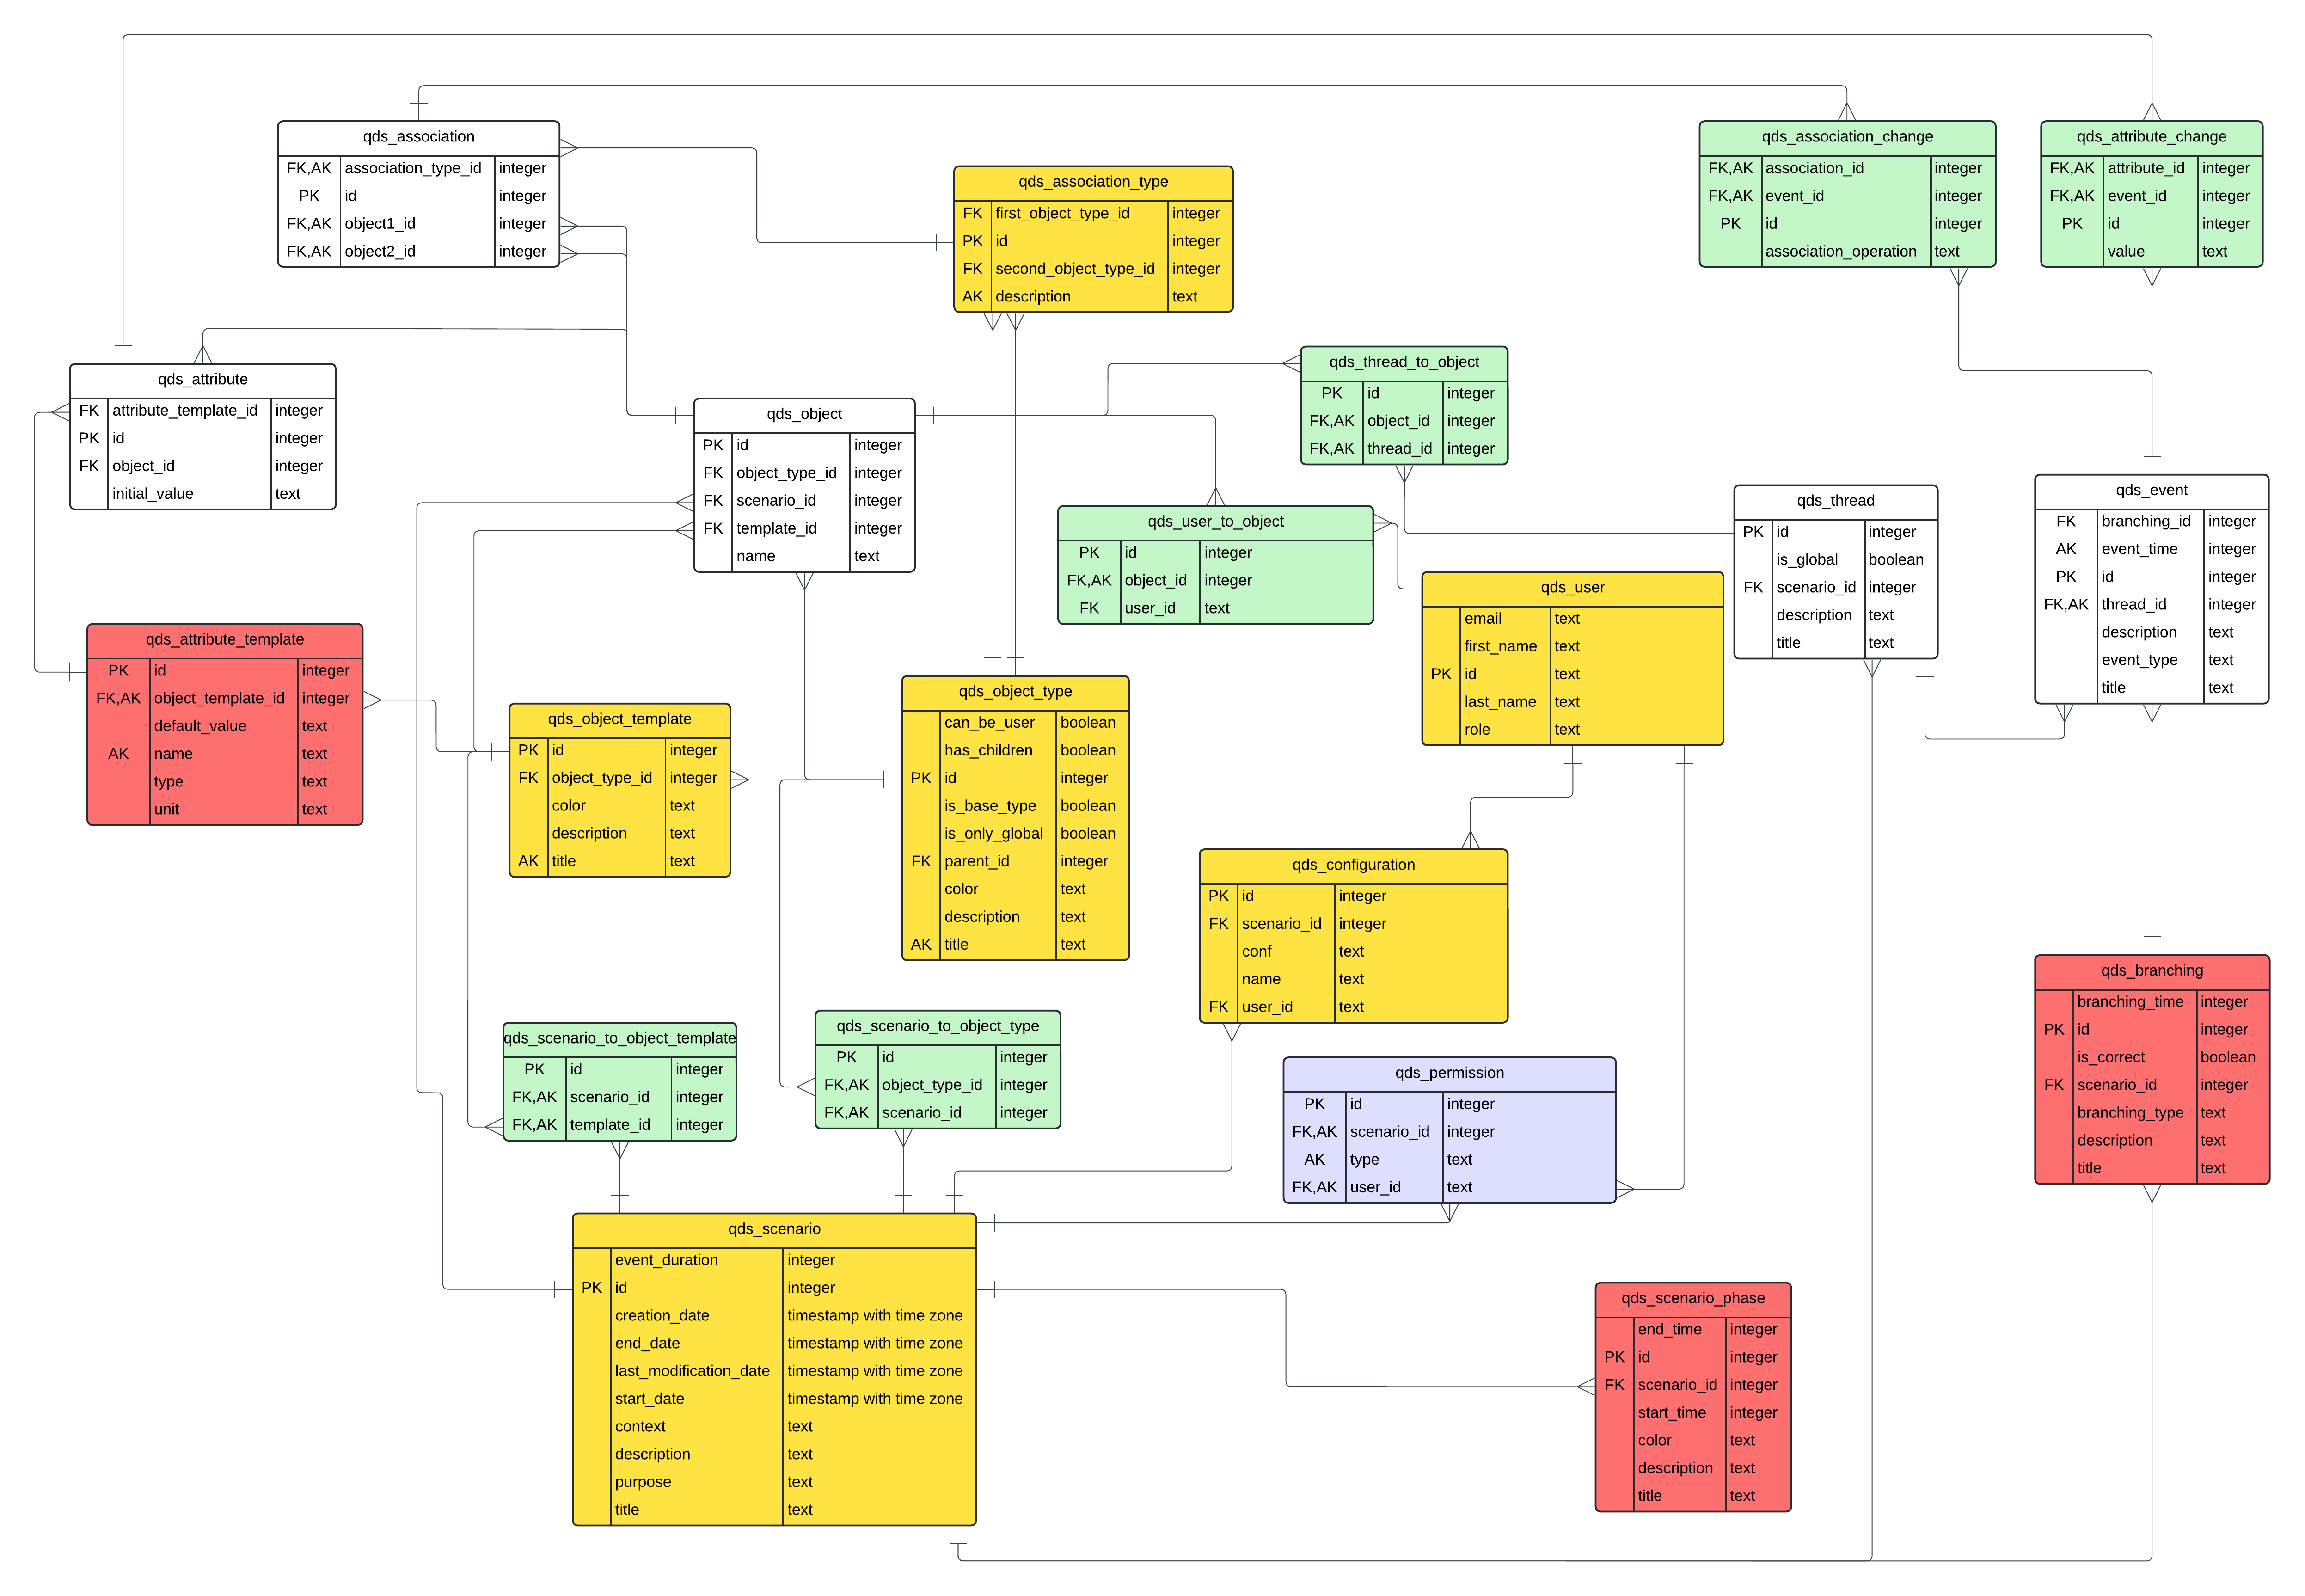
\includegraphics[width=0.99\textwidth]{resources/local/baza-danych-schemat.png}
    \caption{Schemat bazy danych}
\end{figure}

Legenda kolorów:
\begin{itemize}
    \item Żółte - encje globalne współdzielone pomiędzy scenariuszami.
    \item Zielone - encje realizujące relacje wiele do wielu.
    \item Białe - główne encje, które są wyłączne dla każdego scenariusza.
    \item Czerwone - encje pomocnicze.
    \item Niebieski - encje definiujące uprawnienia.
\end{itemize}

\section{Opis encji}

\subsection{Encje scenariuszowe}

\begin{figure}[H]
    \begin{minipage}{\textwidth}
        \centering

        \begin{figure}[H]
            \centering
            \begin{minipage}{0.8\textwidth}
                \begin{framed}
                    \noindent\textbf{\large Nazwa techniczna:} \texttt{qds\_scenario} \\
                    \textbf{\large Nazwa robocza:} Scenariusz \\
                    \textbf{\large Opis:} Reprezentuje scenariusz, centralny element systemu organizujący
                    wydarzenia, wątki i obiekty w określonych ramach czasowych.
                \end{framed}
            \end{minipage}
        \end{figure}


        \begin{table}[H]
            \centering
            \renewcommand{\arraystretch}{1.6}
            \begin{tabular}{|>{\bfseries}l|p{0.7\textwidth}|}
                \hline
                \rowcolor[HTML]{EFEFEF} \textbf{Atrybut} & \textbf{Opis} \\
                \hline
                \texttt{id} & Unikalny identyfikator scenariusza. \\
                \hline
                \texttt{title} & Nazwa scenariusza. \\
                \hline
                \texttt{description} & Opis scenariusza mający przybliżyć najważniejsze informacje na jego temat. \\
                \hline
                \texttt{context} & Kontekst w jakim ma miejsce scenariusz. \\
                \hline
                \texttt{purpose} & Cel przewodni scenariusza. \\
                \hline
                \texttt{event\_duration} & Domyślny czas trwania zdarzenia, wyrażony za pomocą wewnętrznej dla scenariusz jednostki czasu. \\
                \hline
                \texttt{start\_date} & Dokładny moment w czasie rozpoczęcia scenariusza, uwzględniający strefę czasową. \\
                \hline
                \texttt{end\_date} & Dokładny moment w czasie zakończenia scenariusza, uwzględniający strefę czasową. \\
                \hline
                \texttt{creation\_date} & Dokładny moment w czasie utworzenia scenariusza, uwzględniający strefę czasową. \\
                \hline
                \texttt{last\_modification\_date} & Dokładny moment w czasie ostatniej aktualizacji scenariusza, uwzględniający strefę czasową. \\
                \hline
            \end{tabular}
            \caption{Atrybuty encji \texttt{scenariusza}}
        \end{table}
    \end{minipage}
\end{figure}

\begin{figure}[H]
    \begin{minipage}{\textwidth}
        \centering
        \begin{figure}[H]
            \centering
            \begin{minipage}{0.8\textwidth}
                \begin{framed}
                    \noindent\textbf{\large Nazwa techniczna:} \texttt{qds\_scenario\_phase} \\
                    \textbf{\large Nazwa robocza:} Faza scenariusza \\
                    \textbf{\large Opis:} Reprezentuje logiczną fazę czasową w scenariuszu.
                    Fazy pozwalają na podział scenariusza na mniejsze, znaczące okresy, ułatwiając organizację i wizualizację wydarzeń.
                \end{framed}
            \end{minipage}
        \end{figure}

        \begin{table}[H]
            \centering
            \renewcommand{\arraystretch}{1.6}
            \begin{tabular}{|>{\bfseries}l|p{0.8\textwidth}|}
                \hline
                \rowcolor[HTML]{EFEFEF} \textbf{Atrybut} & \textbf{Opis} \\
                \hline
                \texttt{id} & Unikalny identyfikator fazy scenariusza. \\
                \hline
                \texttt{title} & Nazwa fazy scenariusza. \\
                \hline
                \texttt{description} & Opis fazy scenariusza mający przybliżyć najważniejsze informacje na jej temat. \\
                \hline
                \texttt{color} & Kolor zapisany heksadecymalnie, który zostanie użyty podczas wizualizacji fazy. \\
                \hline
                \texttt{start\_date} & Czas rozpoczęcia fazy scenariusza, wyrażony za pomocą wewnętrznej dla scenariusz jednostki czasu. \\
                \hline
                \texttt{end\_date} & Czas zakończenia fazy scenariusza, wyrażony za pomocą wewnętrznej dla scenariusz jednostki czasu. \\
                \hline
                \texttt{scenario\_id} & Klucz obcy scenariusza, do którego należy faza scenariusza. \\
                \hline
            \end{tabular}
            \caption{Atrybuty encji \texttt{fazy scenariusza}}
        \end{table}
    \end{minipage}
\end{figure}

\subsection{Encje konfiguracyjne}

\begin{figure}[H]
    \centering
    \begin{minipage}{0.8\textwidth}
        \begin{framed}
            \noindent\textbf{\large Nazwa techniczna:} \texttt{qds\_user} \\
            \textbf{\large Nazwa robocza:} Użytkownik \\
            \textbf{\large Opis:} Reprezentuje użytkownika systemu. Przechowuje podstawowe informacje o użytkowniku
            oraz jego rolę systemową.
        \end{framed}
    \end{minipage}
\end{figure}

\begin{table}[H]
    \centering
    \renewcommand{\arraystretch}{1.6}
    \begin{tabular}{|>{\bfseries}l|p{0.8\textwidth}|}
        \hline
        \rowcolor[HTML]{EFEFEF} \textbf{Atrybut} & \textbf{Opis} \\
        \hline
        \texttt{id} & Unikalny identyfikator użytkownika. \\
        \hline
        \texttt{email} & Adres e-mail użytkownika. \\
        \hline
        \texttt{first\_name} & Imię użytkownika. \\
        \hline
        \texttt{last\_name} & Nazwisko użytkownika. \\
        \hline
        \texttt{role} & Rola użytkownika:
        \begin{itemize}
            \item \texttt{USER} - Zwykły użytkownik.
            \item \texttt{ADMIN} - Administrator systemu.
        \end{itemize} \\
        \hline
    \end{tabular}
    \caption{Atrybuty encji \texttt{użytkownika}}
\end{table}

\begin{figure}[H]
    \centering
    \begin{minipage}{0.8\textwidth}
        \begin{framed}
            \noindent\textbf{\large Nazwa techniczna:} \texttt{qds\_permission} \\
            \textbf{\large Nazwa robocza:} Permisja \\
            \textbf{\large Opis:} Określa poziomy uprawnień dostępu do scenariusza.
        \end{framed}
    \end{minipage}
\end{figure}

\begin{table}[H]
    \centering
    \renewcommand{\arraystretch}{1.6}
    \begin{tabular}{|>{\bfseries}l|p{0.8\textwidth}|}
        \hline
        \rowcolor[HTML]{EFEFEF} \textbf{Atrybut} & \textbf{Opis} \\
        \hline
        \texttt{id} & Unikalny identyfikator permisji. \\
        \hline
        \texttt{role} & Typ uprawnienia:
        \begin{itemize}
            \item \texttt{AUTHOR} - Pełne uprawnienia, włącznie z zarządzaniem dostępem.
            \item \texttt{EDIT} - Możliwość modyfikacji scenariusza.
            \item \texttt{VIEW} - Podgląd scenariusza.
        \end{itemize} \\
        \hline
        \texttt{scenario\_id} & Klucz obcy scenariusza, do którego odnosi się permisja. \\
        \hline
        \texttt{user\_id} & Klucz obcy użytkownika, do którego odnosi się permisja. \\
        \hline
    \end{tabular}
    \caption{Atrybuty encji \texttt{permisji}}
\end{table}

\begin{figure}[H]
    \centering
    \begin{minipage}{0.8\textwidth}
        \begin{framed}
            \noindent\textbf{\large Nazwa techniczna:} \texttt{qds\_configuration} \\
            \textbf{\large Nazwa robocza:} Konfiguracja \\
            \textbf{\large Opis:} Przechowuje globalne ustawienia konfiguracyjne systemu. Zawiera domyślne wartości
            i parametry wpływające na działanie całego systemu.
        \end{framed}
    \end{minipage}
\end{figure}

\begin{table}[H]
    \centering
    \renewcommand{\arraystretch}{1.6}
    \begin{tabular}{|>{\bfseries}l|p{0.8\textwidth}|}
        \hline
        \rowcolor[HTML]{EFEFEF} \textbf{Atrybut} & \textbf{Opis} \\
        \hline
        \texttt{id} & Unikalny identyfikator konfiguracji. \\
        \hline
        \texttt{name} & Nazwa ustawień, unikalna dla scenariusza oraz użytkownika. \\
        \hline
        \texttt{conf} & Dane konfiguracji przechowywane w formacie JSON. \\
        \hline
        \texttt{scenario\_id} & Klucz obcy scenariusza, do którego odnosi się konfiguracja. \\
        \hline
        \texttt{user\_id} & Klucz obcy użytkownika, do którego odnosi się konfiguracja. \\
        \hline
    \end{tabular}
    \caption{Atrybuty encji \texttt{konfiguracji}}
\end{table}

\subsection{Encje Typów}

\begin{figure}[H]
    \centering
    \begin{minipage}{0.8\textwidth}
        \begin{framed}
            \noindent\textbf{\large Nazwa techniczna:} \texttt{qds\_object\_type} \\
            \textbf{\large Nazwa robocza:} Typ obiektu \\
            \textbf{\large Opis:} Definiuje typ obiektu w systemie, określając jego podstawowe właściwości
            i ograniczenia. Typy mogą tworzyć hierarchię (dziedziczenie) i definiować zasady globalności obiektów.
        \end{framed}
    \end{minipage}
\end{figure}

\begin{table}[H]
    \centering
    \renewcommand{\arraystretch}{1.6}
    \begin{tabular}{|>{\bfseries}l|p{0.8\textwidth}|}
        \hline
        \rowcolor[HTML]{EFEFEF} \textbf{Atrybut} & \textbf{Opis} \\
        \hline
        \texttt{id} & Unikalny identyfikator typu obiektu. \\
        \hline
        \texttt{title} & Unikalny tytuł typu obiektu. \\
        \hline
        \texttt{description} & Opis typu obiektu. \\
        \hline
        \texttt{color} & Kolor zapisany heksadecymalnie, który zostanie użyty podczas wizualizacji obiektu. \\
        \hline
        \texttt{is\_only\_global} & Wartość logiczna stwierdziająca czy obiekt może być tylko w wątku globalnym. \\
        \hline
        \texttt{has\_children} & Wartość logiczna stwierdziająca czy obiekt posiada potomne typy. \\
        \hline
        \texttt{is\_base\_type} & Wartość logiczna stwierdziająca czy jest typem podstawowym, tworzonym przy tworzeniu scenariusza. \\
        \hline
        \texttt{can\_be\_user} & Wartość logiczna stwierdziająca czy obiekt może być przydzielony do użytkownika. \\
        \hline
        \texttt{parent\_id} & Klucz obcy typu nadrzędnego, za pomocą którego tworzy się hierarchia. \\
        \hline
    \end{tabular}
    \caption{Atrybuty encji \texttt{typu obiektu}}
\end{table}

Dodatkowe informacje:
\begin{itemize}
    \item Nie można usunąć typu używanego przez obiekty lub szablony.
    \item Usunięcie typu jest możliwe tylko gdy nie ma typów potomnych.
\end{itemize}

\begin{figure}[H]
    \centering
    \begin{minipage}{0.8\textwidth}
        \begin{framed}
            \noindent\textbf{\large Nazwa techniczna:} \texttt{qds\_association\_type} \\
            \textbf{\large Nazwa robocza:} Typ asocjacji \\
            \textbf{\large Opis:} Definiuje typ/rodzaj asocjacji możliwy między obiektami w systemie.
            Określa jakie typy obiektów mogą być połączone danym rodzajem asocjacji.
        \end{framed}
    \end{minipage}
\end{figure}

\begin{table}[H]
    \centering
    \renewcommand{\arraystretch}{1.6}
    \begin{tabular}{|>{\bfseries}l|p{0.8\textwidth}|}
        \hline
        \rowcolor[HTML]{EFEFEF} \textbf{Atrybut} & \textbf{Opis} \\
        \hline
        \texttt{id} & Unikalny identyfikator typu asocjacji. \\
        \hline
        \texttt{description} & Opis asocjacji \\
        \hline
        \texttt{firstObjectTypeId} & Identyfikator pierwszego dozwolonego typu obiektu. \\
        \hline
        \texttt{secondObjectTypeId} & Identyfikator drugiego dozwolonego typu obiektu. \\
        \hline
    \end{tabular}
    \caption{Atrybuty encji \texttt{typu asocjacji}}
\end{table}

Dodatkowe informacje:
\begin{itemize}
    \item Nie można usunąć używanego typu asocjacji.
    \item Typ obiektu posiada relacje wiele do wielu z encją scenariusza.
\end{itemize}

\subsection{Encje szablonowe}

\begin{figure}[H]
    \centering
    \begin{minipage}{0.8\textwidth}
        \begin{framed}
            \noindent\textbf{\large Nazwa techniczna:} \texttt{qds\_object\_template} \\
            \textbf{\large Nazwa robocza:} Szablon obiektu \\
            \textbf{\large Opis:} Reprezentuje szablon obiektu określający jego strukturę atrybutów.
            Definiuje jakie atrybuty i jakiego typu musi posiadać obiekt stworzony na podstawie tego szablonu.
        \end{framed}
    \end{minipage}
\end{figure}

\begin{table}[H]
    \centering
    \renewcommand{\arraystretch}{1.6}
    \begin{tabular}{|>{\bfseries}l|p{0.8\textwidth}|}
        \hline
        \rowcolor[HTML]{EFEFEF} \textbf{Atrybut} & \textbf{Opis} \\
        \hline
        \texttt{id} & Unikalny identyfikator szablonu obiektu. \\
        \hline
        \texttt{title} & Unikalny tytuł szablonu. \\
        \hline
        \texttt{description} & Opis szablonu. \\
        \hline
        \texttt{color} & Kolor zapisany heksadecymalnie, który zostanie użyty podczas wizualizacji obiektu. \\
        \hline
        \texttt{object\_type\_id} & Klucz obcy typu obiektu, do którego można przypisać szablon. \\
        \hline
    \end{tabular}
    \caption{Atrybuty encji \texttt{szablonu obiektu}}
\end{table}

Dodatkowe informacje:
\begin{itemize}
    \item Nie można usunąć szablonu używanego przez obiekt.
    \item Szablon obiektu posiada relacje wiele do wielu z encją scenariusza.
\end{itemize}

\begin{figure}[H]
    \centering
    \begin{minipage}{0.8\textwidth}
        \begin{framed}
            \noindent\textbf{\large Nazwa techniczna:} \texttt{qds\_attribute\_template} \\
            \textbf{\large Nazwa robocza:} Szablon atrybutu obiektu. \\
            \textbf{\large Opis:} Reprezentuje szablon obiektu określający jego strukturę atrybutów.
            Definiuje jakie atrybuty i jakiego typu musi posiadać obiekt stworzony na podstawie tego szablonu.
        \end{framed}
    \end{minipage}
\end{figure}

\begin{table}[H]
    \centering
    \renewcommand{\arraystretch}{1.6}
    \begin{tabular}{|>{\bfseries}l|p{0.8\textwidth}|}
        \hline
        \rowcolor[HTML]{EFEFEF} \textbf{Atrybut} & \textbf{Opis} \\
        \hline
        \texttt{id} & Unikalny identyfikator szablonu obiektu. \\
        \hline
        \texttt{name} & Unikalna nazwa atrybutu. \\
        \hline
        \texttt{default\_value} & Wartość domyślna atrybutu. \\
        \hline
        \texttt{unit} & Jednostka wartości atrybutu. \\
        \hline
        \texttt{role} & Typ wartości atrybutu:
        \begin{itemize}
            \item \texttt{INT} - liczba całkowita.
            \item \texttt{STRING} - łańcuch znaków.
            \item \texttt{DATE} - data lub czas.
            \item \texttt{BOOL} - wartość logiczna.
        \end{itemize} \\
        \hline
        \texttt{object\_template\_id} & Klucz obcy szablonu obiektu, do którego przydzielony jest atrybut. \\
        \hline
    \end{tabular}
    \caption{Atrybuty encji \texttt{szablonu atrybutu obiektu}}
\end{table}

Dodatkowe informacje:
\begin{itemize}
    \item Usuwany kaskadowo wraz z szablonem obiektu.
\end{itemize}

\subsection{Encje dotyczące konkretnego obiektu}

\begin{figure}[H]
    \centering
    \begin{minipage}{0.8\textwidth}
        \begin{framed}
            \noindent\textbf{\large Nazwa techniczna:} \texttt{qds\_object} \\
            \textbf{\large Nazwa robocza:} Obiekt \\
            \textbf{\large Opis:} Reprezentuje obiekt w scenariuszu, który może być modyfikowany przez wydarzenia.
            Obiekt jest globalny jeśli został utworzony w wątku globalnym, w przeciwnym razie jest lokalny
            i przypisany do konkretnego wątku.
        \end{framed}
    \end{minipage}
\end{figure}

\begin{table}[H]
    \centering
    \renewcommand{\arraystretch}{1.6}
    \begin{tabular}{|>{\bfseries}l|p{0.8\textwidth}|}
        \hline
        \rowcolor[HTML]{EFEFEF} \textbf{Atrybut} & \textbf{Opis} \\
        \hline
        \texttt{id} & Unikalny identyfikator obiektu. \\
        \hline
        \texttt{name} & Unikalna nazwa obiektu. \\
        \hline
        \texttt{object\_type\_id} & Klucz obcy typu obiektu. \\
        \hline
        \texttt{template\_id} & Klucz obcy szablonu obiektu. \\
        \hline
        \texttt{scenario\_id} & Klucz obcy scenariusza obiektu. \\
        \hline
    \end{tabular}
    \caption{Atrybuty encji \texttt{obiektu}}
\end{table}

Dodatkowe informacje:
\begin{itemize}
    \item Obiekt można przypisać do użytkownika systemu.
\end{itemize}

\begin{figure}[H]
    \centering
    \begin{minipage}{0.8\textwidth}
        \begin{framed}
            \noindent\textbf{\large Nazwa techniczna:} \texttt{qds\_association} \\
            \textbf{\large Nazwa robocza:} Asocjacja \\
            \textbf{\large Opis:} Reprezentuje asocjację (relację) między dwoma obiektami w systemie.
            Przechowuje informacje o typie relacji i powiązanych obiektach.
        \end{framed}
    \end{minipage}
\end{figure}

\begin{table}[H]
    \centering
    \renewcommand{\arraystretch}{1.6}
    \begin{tabular}{|>{\bfseries}l|p{0.8\textwidth}|}
        \hline
        \rowcolor[HTML]{EFEFEF} \textbf{Atrybut} & \textbf{Opis} \\
        \hline
        \texttt{id} & Unikalny identyfikator asocjacji. \\
        \hline
        \texttt{association\_type\_id} & Klucz obcy typu asocjacji. \\
        \hline
        \texttt{object1\_id} & Klucz obcy pierwszego obiektu. \\
        \hline
        \texttt{object2\_id} & Klucz obcy drugiego obiektu. \\
        \hline
    \end{tabular}
    \caption{Atrybuty encji \texttt{asocjacji}}
\end{table}

Dodatkowe informacje:
\begin{itemize}
    \item Kombinacja (typ asocjacji, obiekt1, obiekt2) musi być unikalna.
    \item Usuwana automatycznie gdy usuwany jest którykolwiek z obiektów.
\end{itemize}

\begin{figure}[H]
    \centering
    \begin{minipage}{0.8\textwidth}
        \begin{framed}
            \noindent\textbf{\large Nazwa techniczna:} \texttt{qds\_attribute} \\
            \textbf{\large Nazwa robocza:} Atrybut \\
            \textbf{\large Opis:} Reprezentuje atrybut obiektu w systemie wraz z jego wartością początkową.
        \end{framed}
    \end{minipage}
\end{figure}

\begin{table}[H]
    \centering
    \renewcommand{\arraystretch}{1.6}
    \begin{tabular}{|>{\bfseries}l|p{0.8\textwidth}|}
        \hline
        \rowcolor[HTML]{EFEFEF} \textbf{Atrybut} & \textbf{Opis} \\
        \hline
        \texttt{id} & Unikalny identyfikator atrybutu. \\
        \hline
        \texttt{initial\_value} & Wartość początkowa atrybutu. \\
        \hline
        \texttt{object\_id} & Klucz obcy obiektu, którego dotyczy atrybut. \\
        \hline
        \texttt{attribute\_template\_id} & Klucz obcy szablonu atrybutu. \\
        \hline
    \end{tabular}
    \caption{Atrybuty encji \texttt{atrybutu obiektu}}
\end{table}

Dodatkowe informacje:
\begin{itemize}
    \item Każdy obiekt posiada dokładnie wszystkie atrybuty zdefiniowane przez typ obiektu.
    \item Usuwany kaskadowo z obiektem.
\end{itemize}

\subsection{Encje wizualizujące upływ czasu}

\begin{figure}[H]
    \centering
    \begin{minipage}{0.8\textwidth}
        \begin{framed}
            \noindent\textbf{\large Nazwa techniczna:} \texttt{qds\_thread} \\
            \textbf{\large Nazwa robocza:} Wątek \\
            \textbf{\large Opis:} Reprezentuje wątek w scenariuszu - sekwencję wydarzeń w czasie.
        \end{framed}
    \end{minipage}
\end{figure}

\begin{table}[H]
    \centering
    \renewcommand{\arraystretch}{1.6}
    \begin{tabular}{|>{\bfseries}l|p{0.8\textwidth}|}
        \hline
        \rowcolor[HTML]{EFEFEF} \textbf{Atrybut} & \textbf{Opis} \\
        \hline
        \texttt{id} & Unikalny identyfikator wątku. \\
        \hline
        \texttt{title} & Tytuł wątku. \\
        \hline
        \texttt{description} & Opis wątku. \\
        \hline
        \texttt{is\_global} & Wartość logiczna stwierdziająca czy wątek jest globalny, czy lokalny. \\
        \hline
        \texttt{scenario\_id} & Klucz obcy scenariusza. \\
        \hline
    \end{tabular}
    \caption{Atrybuty encji \texttt{wątku}}
\end{table}

\begin{figure}[H]
    \centering
    \begin{minipage}{0.8\textwidth}
        \begin{framed}
            \noindent\textbf{\large Nazwa techniczna:} \texttt{qds\_event} \\
            \textbf{\large Nazwa robocza:} Wydarzenie \\
            \textbf{\large Opis:} Reprezentuje wydarzenie w scenariuszu zachodzące w określonym czasie i wątku.
            Wydarzenia są podstawowym mechanizmem wprowadzania zmian w systemie,
            odpowiadają za modyfikacje atrybutów obiektów i ich asocjacji.
        \end{framed}
    \end{minipage}
\end{figure}

\begin{table}[H]
    \centering
    \renewcommand{\arraystretch}{1.6}
    \begin{tabular}{|>{\bfseries}l|p{0.8\textwidth}|}
        \hline
        \rowcolor[HTML]{EFEFEF} \textbf{Atrybut} & \textbf{Opis} \\
        \hline
        \texttt{id} & Unikalny identyfikator wydarzenia. \\
        \hline
        \texttt{title} & Tytuł wydarzenia. \\
        \hline
        \texttt{description} & Opis wydarzenia. \\
        \hline
        \texttt{event\_time} & czas wydarzenia, wyrażony za pomocą wewnętrznej dla scenariusz jednostki czasu. \\
        \hline
        \texttt{event\_type} & Typ wydarzenia.
        \begin{itemize}
            \item \texttt{GLOBAL} - Wydarzenie w wątku globalnym, nadpisuje zmiany z innych wątków.
            \item \texttt{NORMAL} - Standardowe wydarzenie w wątku.
            \item \texttt{START} - Początek wątku.
            \item \texttt{END} - Koniec wątku.
            \item \texttt{IDLE} - Wydarzenie puste.
            \item \texttt{JOIN\_OUT} - Początek wątku powstałego z połączenia.
            \item \texttt{JOIN\_IN} - Koniec wątku wchodzącego do połączenia.
            \item \texttt{FORK\_OUT} - Początek wątku powstałego z podziału.
            \item \texttt{FORK\_IN} - Wydarzenie w wątku przed podziałem.
        \end{itemize} \\
        \hline
        \texttt{thread\_id} & Klucz obcy wątku, w ramach którego ma miejsce wydarzenie. \\
        \hline
        \texttt{branching\_id} & Identyfikator powiązanego rozgałęzienia (tylko dla FORK/JOIN). \\
        \hline
    \end{tabular}
    \caption{Atrybuty encji \texttt{wydarzenia}}
\end{table}

\begin{figure}[H]
    \centering
    \begin{minipage}{0.8\textwidth}
        \begin{framed}
            \noindent\textbf{\large Nazwa techniczna:} \texttt{qds\_attribute\_change} \\
            \textbf{\large Nazwa robocza:} Zmiana atrybutu \\
            \textbf{\large Opis:} Reprezentuje zmianę wartości atrybutu w kontekście wydarzenia.
            Jest częścią historii zmian atrybutów, gdzie każda zmiana jest powiązana
            z konkretnym wydarzeniem (QdsEvent) określającym kiedy nastąpiła.
        \end{framed}
    \end{minipage}
\end{figure}

\begin{table}[H]
    \centering
    \renewcommand{\arraystretch}{1.6}
    \begin{tabular}{|>{\bfseries}l|p{0.8\textwidth}|}
        \hline
        \rowcolor[HTML]{EFEFEF} \textbf{Atrybut} & \textbf{Opis} \\
        \hline
        \texttt{id} & Unikalny identyfikator zmiany atrybutu. \\
        \hline
        \texttt{value} & Nowa wartość atrybutu. \\
        \hline
        \texttt{attribute\_id} & Klucz obcy atrybutu obiektu, którego wartość ulega zmianie. \\
        \hline
        \texttt{event\_id} & Klucz obcy wydarzenia, w ramach którego odbywa się zmiana atrybutu. \\
        \hline
    \end{tabular}
    \caption{Atrybuty encji \texttt{zmiany atrybutu obiektu}}
\end{table}

Dodatkowe informacje:
\begin{itemize}
    \item Każda zmiana musi być unikalna dla pary (wydarzenie, atrybut).
    \item Zmiany są usuwane kaskadowo wraz z wydarzeniem lub modyfikowanym atrybutem.
\end{itemize}

\begin{figure}[H]
    \centering
    \begin{minipage}{0.8\textwidth}
        \begin{framed}
            \noindent\textbf{\large Nazwa techniczna:} \texttt{qds\_association\_change} \\
            \textbf{\large Nazwa robocza:} Zmiana asocjacji \\
            \textbf{\large Opis:} Reprezentuje zmianę stanu asocjacji (dodanie/usunięcie) w określonym momencie czasu.
            Jest częścią historii zmian asocjacji, gdzie każda zmiana jest powiązana z konkretnym
            wydarzeniem określającym kiedy i w jakim kontekście nastąpiła.
        \end{framed}
    \end{minipage}
\end{figure}

\begin{table}[H]
    \centering
    \renewcommand{\arraystretch}{1.6}
    \begin{tabular}{|>{\bfseries}l|p{0.8\textwidth}|}
        \hline
        \rowcolor[HTML]{EFEFEF} \textbf{Atrybut} & \textbf{Opis} \\
        \hline
        \texttt{id} & Unikalny identyfikator zmiany asocjacji. \\
        \hline
        \texttt{association\_operation} & Rodzaj operacji
        \begin{itemize}
            \item \texttt{INSERT} - Dodanie nowej asocjacji między obiektami.
            \item \texttt{DELETE} - Usunięcie istniejącej asocjacji między obiektami.
        \end{itemize} \\
        \hline
        \texttt{association\_id} & Klucz obcy atrybutu obiektu, którego wartość ulega zmianie. \\
        \hline
        \texttt{event\_id} & Klucz obcy wydarzenia, w ramach którego odbywa się zmiana atrybutu. \\
        \hline
    \end{tabular}
    \caption{Atrybuty encji \texttt{zmiany asocjacji obiektu}}
\end{table}

Dodatkowe informacje:
\begin{itemize}
    \item Każda zmiana musi być unikalna dla pary (wydarzenie, asocjacja).
    \item Zmiany są usuwane kaskadowo wraz z wydarzeniem lub modyfikowaną asocjacją.
\end{itemize}

\section{Indeksy}

Indeks to struktura danych, pozwalająca na przyśpieszenie operacji odczytu w bazie danych.
Poprzez wygenerowaną strukturę danych, operacja szukania odpowiednich rekordów posiada o wiele mniejszą złożoność.
W naszym przypadku używamy indeksów HASH, ponieważ najlepiej sprawdzają się w operacjach równościowych.
Klucze są unikalne, co znacznie zmniejsza prawdopodobieństwo kolizji. Dodatkowo, kolejność
nie jest istotna w kolumnach identyfikujących.

\begin{itemize}
    \item \textbf{Tabela:} \texttt{qds\_scenario\_phase}, \textbf{Kolumna:} \texttt{scenario\_id}
    Indeks optymalizujący wyszukiwanie faz scenariusza po identyfikatorze scenariusza.

    \item \textbf{Tabela:} \texttt{qds\_association\_type}, \textbf{Kolumna:} \texttt{first\_object\_type\_id}
    Indeks przyspieszający wyszukiwanie asocjacji po pierwszym typie obiektu.

    \item \textbf{Tabela:} \texttt{qds\_association\_change}, \textbf{Kolumna:} \texttt{association\_id}
    Indeks optymalizujący wyszukiwanie zmian danej asocjacji.

    \item \textbf{Tabela:} \texttt{qds\_attribute\_change}, \textbf{Kolumna:} \texttt{event\_id}
    Indeks przyspieszający wyszukiwanie zmian atrybutów związanych z określonym wydarzeniem.

    \item \textbf{Tabela:} \texttt{qds\_object}, \textbf{Kolumna:} \texttt{scenario\_id}
    Indeks zapewniający unikalność obiektów w scenariuszu.

    \item \textbf{Tabela:} \texttt{qds\_thread}, \textbf{Kolumna:} \texttt{scenario\_id}, \textbf{Warunek:} \texttt{is\_global = TRUE}
    Unikalny indeks zapewniający, że w danym scenariuszu może istnieć tylko jeden wątek globalny.

    \item \textbf{Tabela:} \texttt{qds\_thread}, \textbf{Kolumna:} \texttt{scenario\_id}
    Indeks optymalizujący wyszukiwanie wątków scenariusza.

    \item \textbf{Tabela:} \texttt{qds\_branching}, \textbf{Kolumna:} \texttt{scenario\_id}
    Indeks przyspieszający wyszukiwanie rozgałęzień danego scenariuszu.

    \item \textbf{Tabela:} \texttt{qds\_event}, \textbf{Kolumna:} \texttt{thread\_id}
    Indeks optymalizujący wyszukiwanie wydarzeń danego wątku.
\end{itemize}

    
\chapter{Implementacja}

\section{REST API}
REST API jest to interfejs służący do komunikacji między Backendem i Frontendem, przez to realizując architekturę klient-serwer. W naszym projekcie został zaimplementowany 
za pomocą frameworka Spring Boot. Dzięki niemu możliwa była wydajna i prosta integracja z bazą danych PostgreSQL, która jest istotnym
punktem naszego systemu. Użycie Spring Boota umożliwiło zastosowanie operacji CRUD, które z kolei są możliwe do implementacji dzięki 
metodom HTTP takim jak: GET, PUT, POST, DELETE. Ważna cecha jaką jest warstwowość pozwoliła nam na oddzielenie części aplikacji:
\begin{itemize}
    \item Warstwa prezencji - składa się z kontrolerów, z których zarówno może korzystać frontend oraz inne serwisy.
    \item Warstwa serwisowa - składająca się z serwisów, które odpowiadają za logikę biznesową aplikacji.
    \item Warstwa dostępu do danych - składają się z repozytoriów, które odpowiadają za operacje na bazie danych.
    \item Warstwa infastrukturalna - składająca się z wielu komponentów, odpowiedzialnych głównie za konfigurację oraz kontakt z zewnętrznymi
    serwisami.
\end{itemize}

Wszystkie endpointy zabezpieczone są za pomocą tokenów JWT, dzięki czemu unikamy nieautoryzowanego dostępu do danych. 

Poszczególne błędy walidacyjne, lub z warstwy serwisowej oraz bazodanowej, wychwytywane są przez dedykowane handlery, które zapewniają ustandaryzowaną odpowiedź w formacie JSON wraz z
odpowiednim kodem statusu HTTP. 

Dla endpointów z potencjałem na zwracanie bardzo dużej ilości danych dodaliśmy mechanizm paginowania. Odpowiedzi dzielone są na strony 
co znacznie usprawnia wydajność przesyłania danych.

\begin{figure}[h!]
    \centering
    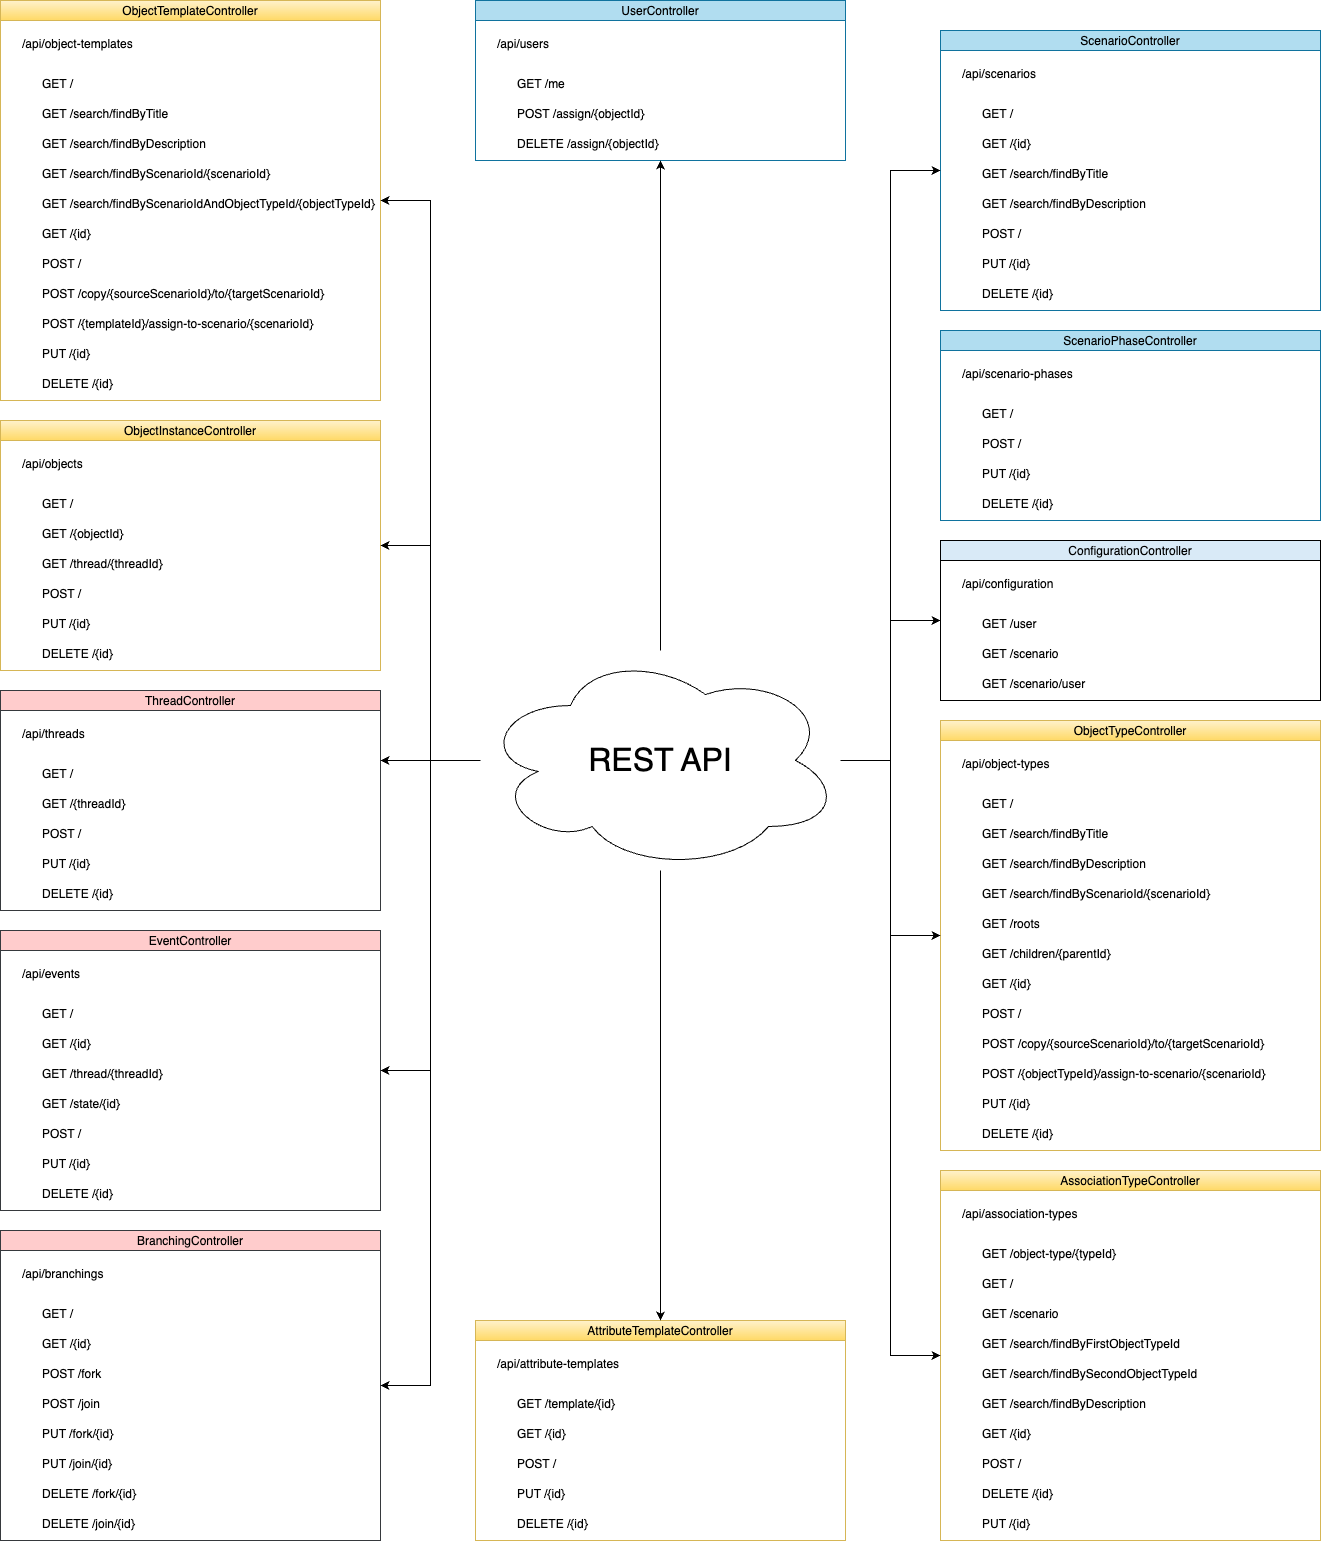
\includegraphics[width=0.99\textwidth]{resources/local/diagram-api.png}
    \caption{Diagram REST API}
\end{figure}

\section{Backend}

\subsection{Autoryzacja oraz uprawnienia}

Autoryzacja w naszej aplikacji obejmuje wszystkie endpointy, z wyjątkiem tych zdefiniowanych w liście odstępstw:
\begin{itemize}
    \item Autoryzacja i zdarzenia z keycloacka,
    \item Dokumentacja,
    \item Monitorowanie stanu aplikacji.
\end{itemize}
Odbywa się ona za pomocą tokenów JWT. Znajduje się on w kontekście bezpieczeństwa danego requesta, w obiekcie Authentication.
Dzięki danym znajdującym się w tokenie oraz wymaganym nagłówku posiadającym id scenariusza możemy sprawdzić czy użytkownik posiada uprawnienia edycji 
lub modyfikacji konkretnego scenariusza. Ważnym elementem architektury bezpieczeństwa naszej aplikacji jest CORS. 
Zablokuje on jakiekolwiek połączenia z niezdefiniowanych przez nas domen. Znacznie zwiększa to bezpieczeństwo aplikacji. 
w konfiguracja CORS-a definiujemy akceptowalne domeny, metody HTTP oraz nagłówki. W konfiguracji określamy także, że 
nie tworzymy oraz utrzymuje sesji HTTP dla użytkowników, ponieważ nie jest to potrzebne w sytuacji gdy wykorzystujemy mechanizm
tokenów. Za każdym razem posiadamy potrzebne dane autoryzacyjne. Wyłączamy także ochronę przed atakiem CSRF, która to jest domyślnie 
ustawiona w Spring Boot. Taki atak nie jest zagrożeniem w naszej polityce zarządzania sesjami.

Zdefiniowanie oddzielnych profili: deweloperskiego oraz produkcyjnego, pozwoliło nam na złagodzenie wielu warunków autoryzacyjnych
w sytuacji lokalnego uruchomienia aplikacji. 

\subsection{Obsługa błędów}

Błędy zwracane przez aplikację backendową wyglądają w następujący sposób:

\begin{lstlisting}[language=Java]
{
  "errorCode": "PHASE_OVERLAP",
  "errorGroup": "SCENARIO_PHASE",
  "values": ["12345"]
}
\end{lstlisting}

Wyjaśnienie poszczególnych części zwracanych błędów:
\begin{itemize}
    \item errorCode - klasa enum (wyliczeniowa), która zawiera w sobie szczegółowy kod błędu. Możemy ją potraktować jako
    ustandaryzowaną wiadomość wyjątku.
    \item errorGroup - klasa enum (wyliczeniowa), która mówi o tym z jaką częścią zapytania jest problem. Najczęściej odnosi się
    do konkretnej encji w bazie danych z nielicznymi wyjątkami.
    \item values - opcjonalna lista wartości kontekstowych, które można załączyć do błedu np. id obiektu w bazie. Ułatwia detekcje 
    problematycznego elementu.
\end{itemize}

W aplikacji posiadamy handlery, które odpowiadają za wychwytywanie błędów i transformowanie ich do jednolitej formy.
Możemy wyróżnić następujące typy handlerów:
\begin{itemize}
    \item bazodanowe - wychwytywanie błędów z bazy danych. Dopasowywujemy error code oraz error group na podstawie wiadomości wyjątku. Gdy dopasowanie nie
    jest możliwe zwracamy błąd serwera.
    \item walidacyjne - wychwytywanie błędów wynikających z błednych lub brakujących danych w requeście.
    \item biznesowe - wychwytywanie błędów rzucanych w warstwie biznesowej.
\end{itemize}

\subsection{Repozytoria}

Warstwa dostępu do danych, w naszej aplikacji, realizowana jest za pomocą repozytoriów JPA (Java Persistence API) dla poszczególnych encji. 
Takie podejście zapewnia gotowe funkcje CRUD, wspiera transakcje oraz umożliwia prostą implementację sortowania oraz paginacji.
Dla bardziej zaawansowanych zapytań stosujemy zapytania SQL. Pozwala nam na zejście z wysokiego poziomu abstrakcji, i operowanie
bezpośrednio na bazie danych.

\subsection{Walidacja danych}

Walidacja w naszym projekcie odbywa się na trzech warstwach: na poziome żądań, w logice biznesowej oraz bazie danych.
Pierwszy typ walidowania danych żądania realizujemy poprzez użycie biblioteki Jakarta Bean Validation. Umożliwia ona w prosty
i czytelny sposób oznaczać poszczególne atrybuty żądania za pomocą adnotacji. Przykładowy kod wykorzystujący tę bibliotekę
wygląda w następujący sposób:

\begin{lstlisting}[language=Java]
public record EventUpdateRequest(
  @NotNull(message = "NULL_VALUE;EVENT;description") String description,
  @NotNull(message = "NULL_VALUE;EVENT;title") String title,
  @NotNull(message = "NULL_VALUE;EVENT;associationChanges")
  @Valid
  List<AssociationChangeData> associationChanges,
  @NotNull(message = "NULL_VALUE;EVENT;attributeChanges")
  @Valid
  List<AttributeChangeData> attributeChanges
) {}
\end{lstlisting}

Jak widać w ukazanym kodzie adnotacja składa się z warunku, oraz wiadomości błędu zwracanej gdy dany wymaganie nie zostanie 
spełnione. Ponadto, dzięki użyciu adnotacji @Valid w stosunku do złożonych obiektów umożliwiamy hierarchiczną walidację.
Kolejnym istotnym aspektem jest użycie recordów, jako rodzaj klasy za pomocą której reprezentujemy dane wejściowe. Jest to stosunkowo
nowa funkcjonalność w języku Java, która ma na celu realizować rolę prostego nośnika danych. Ich główne zalety to:
\begin{itemize}
    \item Minimalizacja kodu,
    \item Niemutowalność,
    \item Poprawa czytelności kodu.
\end{itemize}

Do drugiego typu walidacji żądania wymagane są istniejące dane z bazy danych. Dobrym przykładem takiej walidacji jest transfer 
obiektów podczas rozdziału wątków. Musimy sprawdzić czy wszystkie obiekty zostały przeniesione do nowo utworzonych wątków, oraz 
czy obiekty związane razem asocjacją znajdują się w tym samym wątku. Za tego typu walidacje odpowiadają przeznaczone serwisy.

Ostatnim etapem walidacji żądania jest baza danych. W tym etapie wychwytywane są błędy zgłaszane przez bazę danych, oraz zmienianie
na wewnętrzny model błędu. Przykładowymi wyłapywanymi błędami z bazy danych są: brak klucza obcego, wartość NULL w kolumnie oznaczonej
jako NOT NULL lub naruszenie klucza obcego podczas usuwania obiektu. 

\subsection{Websocket}

Todo: napisać jak osiągnie ostateczną wersję

\subsection{Testy}

W aplikacji zaimplementowane zostały testy integracyjne oraz jednostkowe. Obydwa typy testów posiadają swoją bazową klasę
konfiguracyjną, która odpowiada za stworzenie bazy danych przy pomocy Testcontainers oraz wstrzyknięcie zależności przydatnych
w większości testów. Przykładem takiej zależności jest MockMvc, który umożliwia symulowanie żądań HTTP do kontrolerów.

Pokrycie endpointów testami wynosi 90\%. Dla nieprzetestowanych endpointów lepsze zastosowanie miały testy jednostkowe z powodu
skomplikowanej logiki biznesowej. Dla endpointów GET sprawdzany jest cały response za pomocą pliku JSON z poprawną odpowiedzią.
Pozostałe endpointy testujemy za pomocą asercji dotyczących stanu bazy danych.

\section{Frontend}
\subsection{Opis}
\subsubsection{Architektura systemu}
Interfejs użytkownika został opracowany w systemie Figma, na podstawie którego powstała aplikacja kliencka wykorzystująca TypeScript wraz z biblioteką React.js jako bazę interfejsu użytkownika.
\subsubsection{Warstwa wizualna i dostępność}
Warstwa wizualna opiera się na bibliotece Radix UI, dostarczającej komponenty typu headless\footnote{Komponenty headless to elementy interfejsu użytkownika pozbawione własnej warstwy prezentacji, dostarczające wyłącznie logikę działania i zachowania.}. Komponenty zaimplementowano przy użyciu biblioteki shadcn/ui, która dostarcza wzorce implementacji rozwiązań Radix UI do modyfikacji pod potrzeby zastosowań. Do stylizacji wykorzystano framework TailwindCSS. System dostosowuje interfejs do urządzeń mobilnych oraz stacjonarnych, zachowując standardy WCAG oraz wsparcie dostępności.

\subsubsection{Nawigacja i struktura aplikacji}
Panel boczny stanowi główny element nawigacyjny, adaptujący zawartość do kontekstu aplikacji. W katalogu scenariuszy zawiera nawigację wraz z listą ostatnio używanych scenariuszy. Panel zarządzania kontem znajduje się w dolnej części interfejsu.
Stan aplikacji oraz wyświetlanie paneli przechowywane są w parametrach URL\footnote{Część adresu URL po znaku zapytania, pozwalająca na przechowywanie stanu aplikacji w sposób umożliwiający nawigację przy użyciu funkcji przeglądarki}. Zapewnia to integrację z mechanizmami nawigacji przeglądarki.
\subsubsection{System powiadomień i obsługi błędów}
System powiadomień informuje użytkownika o statusie operacji API, błędach oraz ostrzeżeniach. Akcje użytkownika wyświetlają wskaźniki stanu ładowania. System obsługi błędów wznawia nieudane operacje API.

\subsubsection{Mechanizmy interakcji}
Aplikacja wykorzystuje nawigację klawiaturową oraz skróty klawiszowe dla wykonywanych akcji. Skróty obejmują dostęp do wyszukiwarki, nawigację po formularzach oraz operacje w edytorze scenariuszy. Elementy interakcji, przyciski akcji, formularze z walidacją oraz menu kontekstowe zachowują spójne działanie.
Formularze dialogowe wyposażone są w przycisk rozwijania zawartości w prawym górnym rogu. W trybie zwiniętym, pola posiadające dodatkowe informacje oznaczone są ikoną znaku zapytania. Po najechaniu kursorem na ikonę wyświetlana jest podpowiedź dotycząca danego pola. W trybie rozwiniętym, opisy pól prezentowane są w formie tekstu po lewej stronie formularza.

\subsubsection{Integracja z systemem}
Aplikacja wykorzystuje bibliotekę Keycloak.js do zarządzania stanem autoryzacji i komunikacji z serwerem uwierzytelniania. System działa jako oddzielna usługa, przekazując dane użytkownika. Dostęp do elementów aplikacji wymaga autoryzacji przez ten system.


Aplikacja używa interfejsu REST opisanego systemu backendowego. Do zarządzania stanem danych z API wykorzystano bibliotekę TanStack Query.

\subsection{Katalog scenariuszy}

Katalog scenariuszy stanowi główną stronę aplikacji, na którą następuje przekierowanie po autoryzacji. Z poziomu panelu bocznego dostępny jest katalog obiektów biblioteki oraz lista ostatnio edytowanych scenariuszy.

\begin{figure}[h]
    \centering
    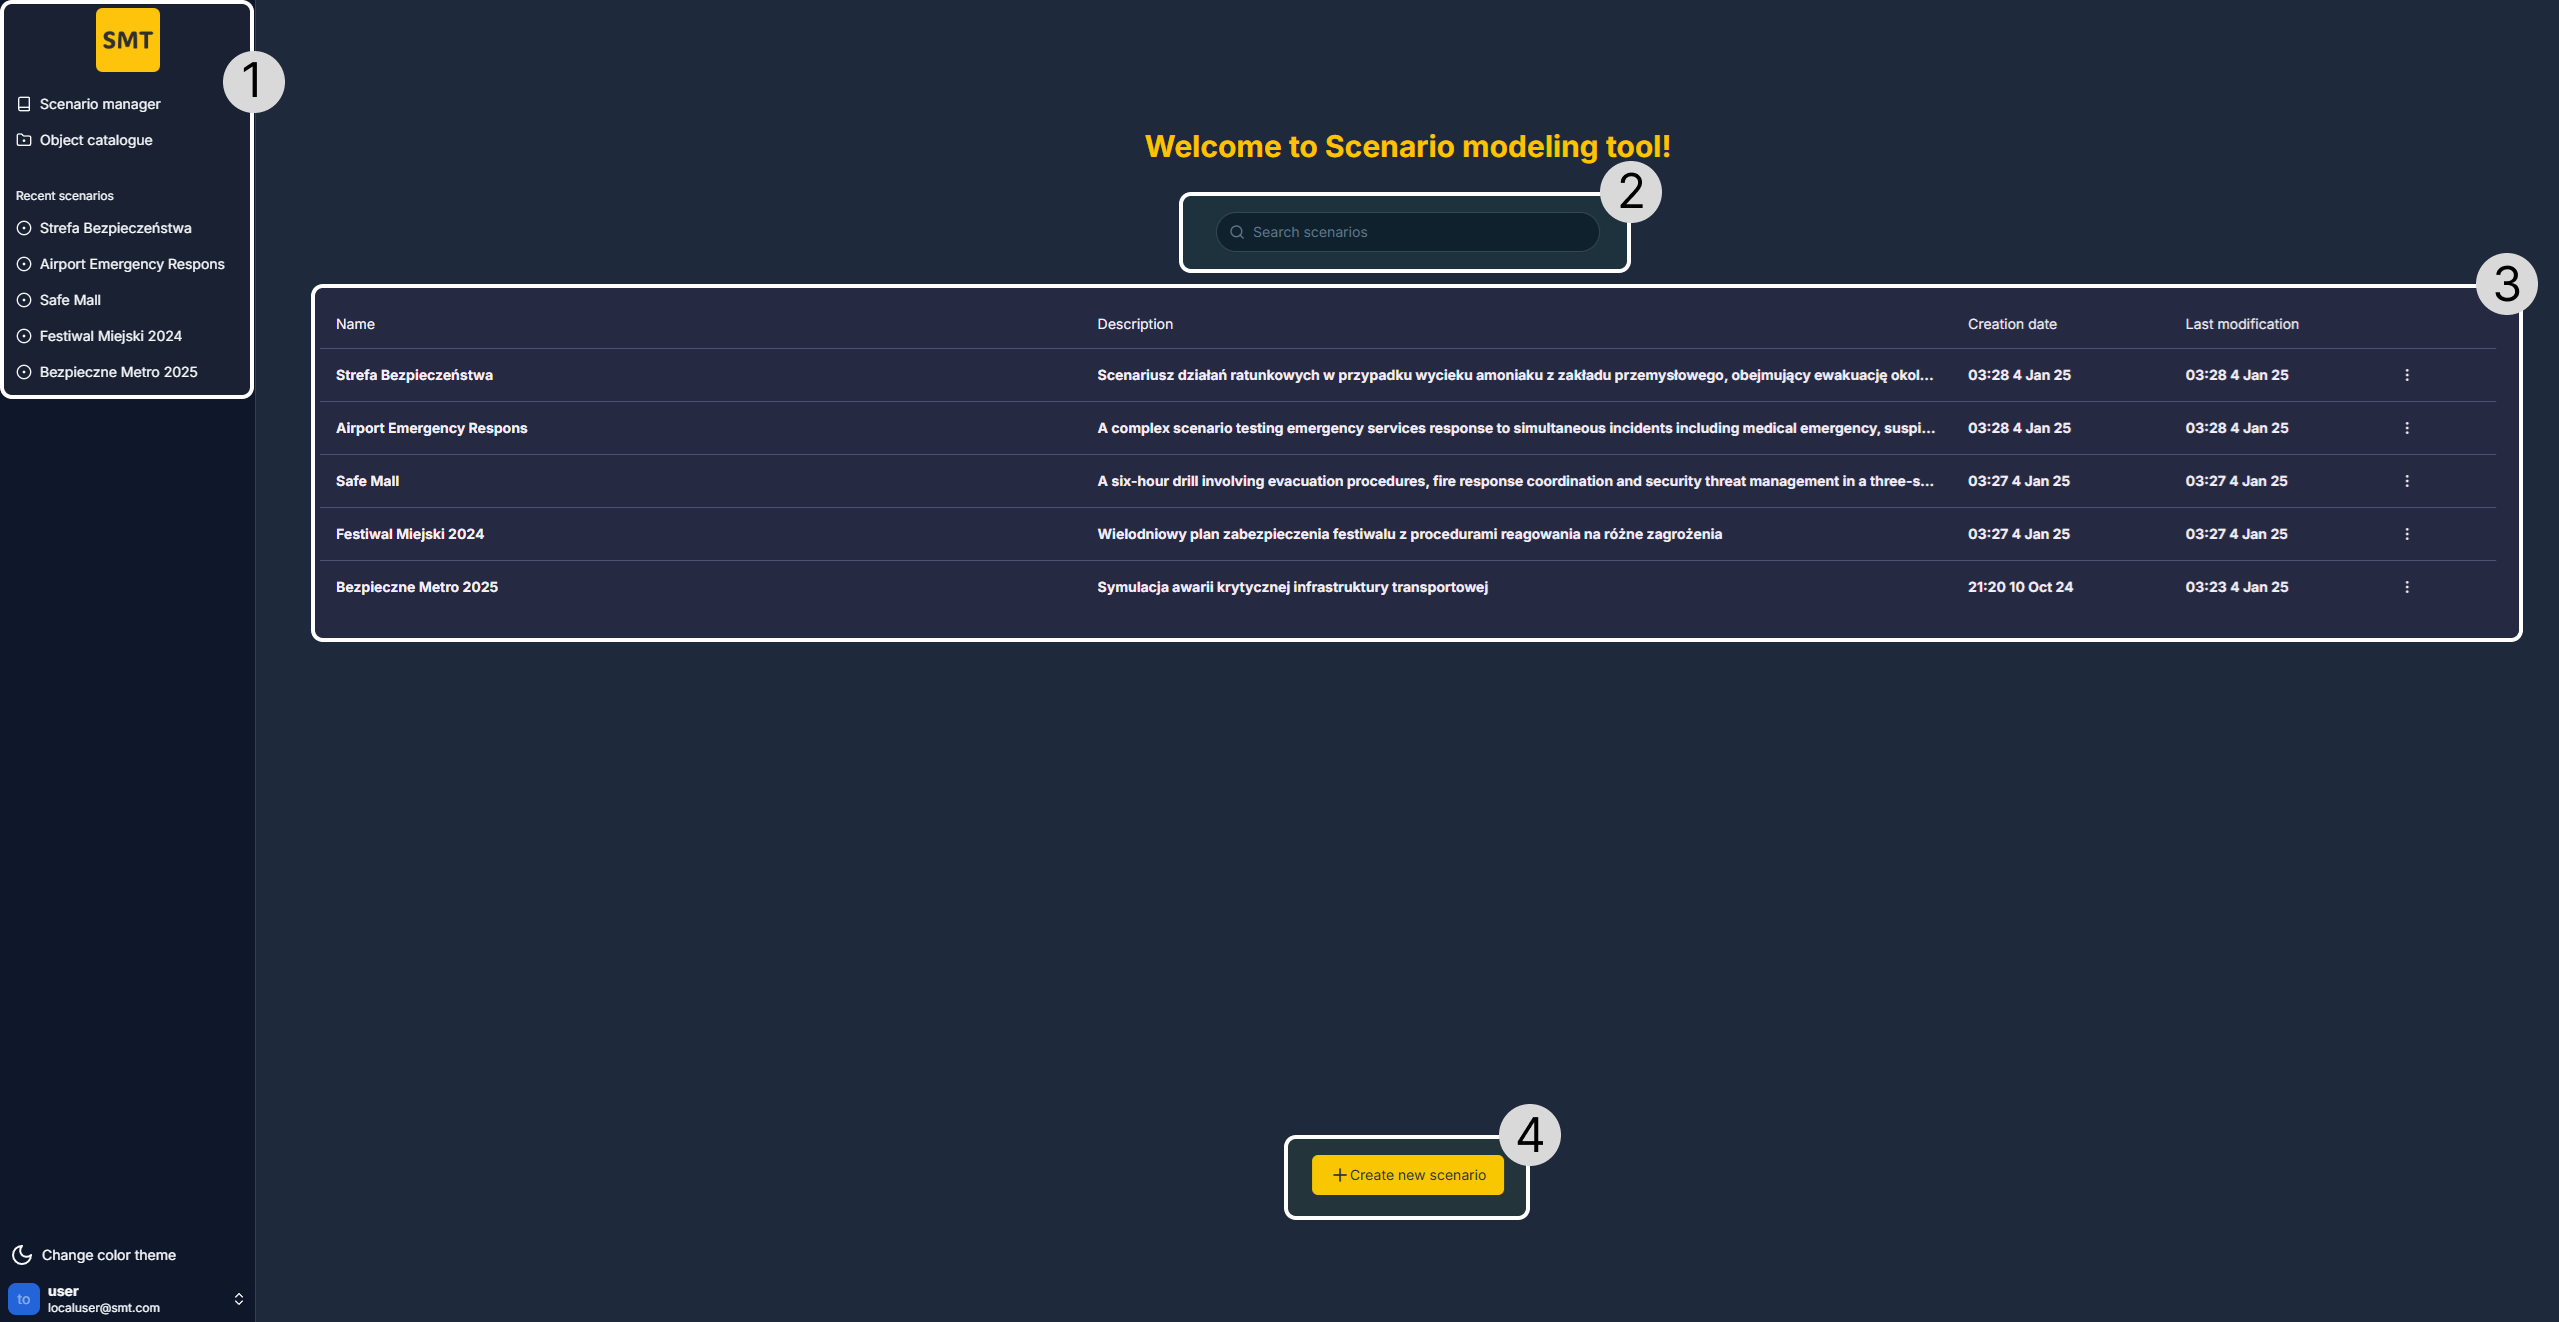
\includegraphics[width=\textwidth]{resources/local/04-implementacja/frontend/landing/landing-page-filled}
    \caption{Widok katalogu scenariuszy}
    \label{fig:scenario_manager}
\end{figure}

Strona ta składa się z czterech głównych elementów funkcjonalnych. 
Panel boczny pełni rolę głównego narzędzia nawigacyjnego systemu, pozwalając na szybkie przełączanie między menedżerem scenariuszy a katalogiem obiektów biblioteki. W jego dolnej części znajduje się sekcja szybkiego dostępu do ostatnio edytowanych scenariuszy oraz panel zarządzania kontem użytkownika.


Centralna część interfejsu zawiera pole wyszukiwania, umożliwiające filtrowanie wyświetlanych scenariuszy w czasie rzeczywistym na podstawie wprowadzanej nazwy. Poniżej znajduje się tabela scenariuszy, prezentująca listę wszystkich dostępnych w systemie scenariuszy.
W dolnej części interfejsu umieszczono przycisk tworzenia nowego scenariusza, który inicjuje proces dodawania nowego scenariusza do systemu.

Posumowując interfejs, ten składa się z następujących elementów:
\begin{enumerate}
    \item Panel boczny z dostępem do funkcji systemu.
    \item Pole wyszukiwania scenariuszy.
    \item Tabela scenariuszy z informacjami o nazwie, opisie i datach modyfikacji.
    \item Przycisk tworzenia nowego scenariusza.
\end{enumerate}

\subsubsection{Tabela scenariuszy}
Tabela prezentuje graficzną reprezentację encji qds\textunderscore scenario, wyświetlając dla każdego scenariusza skrócony tytuł, opis oraz sformatowane daty utworzenia i ostatniej modyfikacji. Po przekroczeniu 10 elementów, aktywuje się system paginacji z nawigacją między stronami wyników.
Interakcja z poszczególnymi scenariuszami możliwa jest poprzez kliknięcie lewym przyciskiem myszy, co prowadzi do edytora scenariusza. Dodatkowe opcje edycji i usunięcia scenariusza dostępne są zarówno przez menu rozwijane z prawej strony wiersza, jak i przez menu kontekstowe wywoływane prawym przyciskiem myszy. Oba menu zawierają identyczny zestaw funkcji.
\begin{figure}[h]
    \centering
    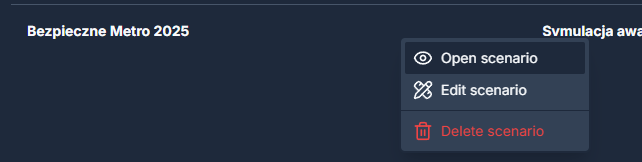
\includegraphics[width=\textwidth]{resources/local/04-implementacja/frontend/landing/context-menu}
    \caption{Menu kontekstowe scenariusza}
\end{figure}

\subsubsection{Formularz tworzenia scenariusza}
\begin{figure}[h]
    \centering
    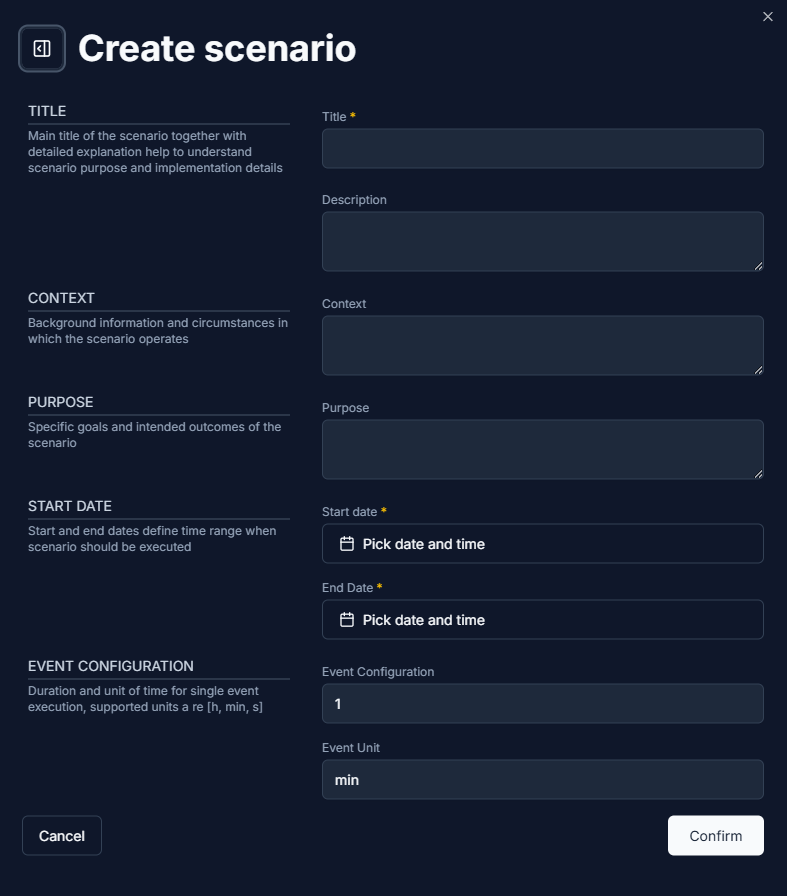
\includegraphics[width=\textwidth]{resources/local/04-implementacja/frontend/landing/create-scenario-form}
    \caption{Rozwinięty formularz tworzenia scenariusza}
    \label{fig:create_scenario}
\end{figure}
Formularz tworzenia nowego scenariusza wyświetlany jest w centralnej części interfejsu, z przyciemnionym tłem aplikacji. Zawiera następujące pola:
\begin{itemize}
    \item Title - główny tytuł scenariusza wraz z opisem szczegółowym (pole wymagane).
    \item Description - opis ogólny scenariusza.
    \item Context - informacje o tle i okolicznościach wykonywania scenariusza.
    \item Purpose - cele i zamierzone rezultaty scenariusza.
    \item Start Date i End Date - zakres czasowy wykonania scenariusza (pola wymagane).
    \item Event Configuration - konfiguracja czasu pojedynczego wydarzenia z wyborem jednostki czasu (h, min, s).
\end{itemize}
W rozwiniętej formie formularza, wszystkie opisy pól widoczne są po lewej stronie interfejsu, dostarczając szczegółowych informacji o przeznaczeniu każdego pola.
System Event Configuration pozwala na wybór jednostki czasu (h, min, s) dla pojedynczego wydarzenia. Domyślnie dostępna jest dowolna jednostka, jednak wybór konkretnej jednostki (godziny, minuty lub sekundy) udostępnia dodatkowe opcje konfiguracji specyficzne dla danej jednostki czasu.
Po wypełnieniu formularza dane przesyłane są do backendu poprzez interfejs REST API. Formularz implementuje wstępną walidację danych - przykładowo, jeśli data rozpoczęcia jest późniejsza niż data zakończenia, pod polem Start Date wyświetlany jest komunikat o niemożliwej konfiguracji. W przypadku poprawnej walidacji i pomyślnej odpowiedzi z serwera, formularz zostaje zamknięty, wyświetlane jest powiadomienie o sukcesie, a nowy scenariusz pojawia się na liście. W przypadku błędu zwróconego przez API, system wyświetla odpowiedni komunikat błędu.
Zamknięcie formularza możliwe jest poprzez kliknięcie poza jego obszarem, użycie przycisku Cancel lub klawisza Escape. Zatwierdzenie formularza następuje po kliknięciu przycisku Confirm lub użyciu klawisza Enter.

\subsubsection{Dialog usuwania scenariusza}
\begin{figure}[h]
    \centering
    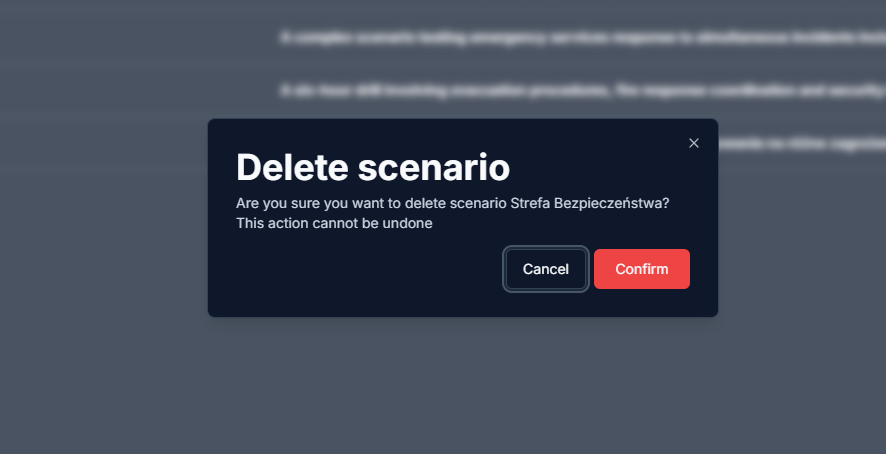
\includegraphics[width=\textwidth]{resources/local/04-implementacja/frontend/landing/delete-scenario-form}
    \caption{Dialog potwierdzenia usunięcia scenariusza}
    \label{fig:delete_scenario}
\end{figure}
Dialog potwierdzenia usunięcia scenariusza wyświetlany jest po wybraniu opcji usunięcia z menu kontekstowego lub rozwijanego. Zawiera on informację ostrzegawczą o nieodwracalności operacji wraz z nazwą usuwanego scenariusza oraz przyciski Cancel i Confirm.
Po zatwierdzeniu, wysyłane jest żądanie do API, a użytkownik informowany jest o statusie operacji poprzez system powiadomień. Podobnie jak w przypadku innych formularzy, dialog można zamknąć poprzez kliknięcie poza jego obszarem, użycie przycisku Cancel lub klawisza Escape.

    \input{chapters/05-zapewnienie-jakości}
    \input{chapters/06-doświadczenia}
    \chapter{Możliwy przyszły rozwój aplikacji}

W tym rozdziale wskazano potencjalne kierunki rozwoju aplikacji. Wymienione funkcjonalności wpłynełyby pozytywnie za równo na
możliwości użytkownika, jakość tworzonych scenariuszy oraz łatwość współpracy.

\section{Perspektywy}

Wizualizacja danych z różnych punktów widzenia:
\begin{itemize}
    \item Koordynator - wizualizacja całościowej realizacji scenariusza na poziomie faz i wątków. Dobrym sposobem wizualizacji tej
    perspektywy jest wykres Gantta.
    \item Aktor - wizualizacja wątków i obiektów istotnych dla konkretnego aktora.
    \item Obserwator w konkretnej lokalizacji - wizualizacja wątków i obiektów istotnych dla całego scenariusza oraz konkretnej fizycznej lokalizacji.
\end{itemize}

Ułatwiłoby to użytkownikom systemu zrozumienie ich roli, oraz ograniczyło zakres scenariusza do informacji im potrzebnych.

\section{Zdarzenia alternatywne}

W naszej implementacji zdarzenie 
może wpłynąć na asocjacje oraz atrybuty obiektów tylko w jeden wybrany sposób. Zdarzenia alternatywne polegałyby na 
zapoczątkowaniu kilku nowych alternatywnych ścieżek fabuły. 
\noindent Jako przykład można wskazać dwie sytuacje:
\begin{itemize}
    \item Uczniowie ewakuowali się na dach.
    \item Uczniowie ewakuowali się do piwnicy.
\end{itemize}
\noindent Po takim zdarzeniu tworzyłyby się nowe alternatywne wątki. Różni się to od aktualnej implementacji wątków, 
ponieważ obecnie umożliwiają one ukazanie równoległych, a nie alternatywnych, zdarzeń.

\section{Moduł ewaluacji ćwiczeń}

Moduł ewaluacji umożliwiłby realizację kolejnego etapu ćwiczeń, czyli analizę i ocenę odbytych ćwiczeń. Opierałby się na 
wykorzystaniu perspektywy obserwatora, który mógłby prowadzić ocenę na poziomie wykonania poszczególnych akcji. 
Wynikiem tych działań byłby całościowy raport oceniający skuteczność przeprowadzonych ćwiczeń,
wskazujący miejsca do poprawy oraz wyciągnięte wnioski.


\section{Zarządzanie wielodostępem}

Przydatny byłby mechanizm proponowania zmian dla właściciela scenariusza. Użytkownik z wyłącznym prawem do odczytu mógłby proponować 
zmiany właścicielowi scenariusza. Dodatkowo, dobrze współgrałby z tym mechanizm perspektywy. Podzielono by scenariusz na części, 
za które odpowiedzialni by byli różni użytkownicy. Prawa odczytu i zmiany dotyczyłyby części scenariusza, a nie tak jak aktualnie 
całości.

\section{Eksport scenariusza}

Dużym usprawnieniem byłaby możliwość eksportu scenariusza do szeroko używanego formatu pliku jak np. XML.
Ułatwiłoby to wymianę informacji pomiędzy organizacjami oraz systemami. Takie rozwiązanie wspiera automatyzację procesów,
oraz zgodność z panującymi standardami.
    \input{chapters/08-zakończenie}

%--------------------------------------
% Literatura
%--------------------------------------

    \begin{thebibliography}{99}

    \bibitem[1]{cleancode}
    Robert C. Martin. \emph{Clean Code: A Handbook of Agile Software Craftsmanship}. Pearson, 2008. \url{https://cleancodebook.com/}.

    \bibitem[2]{scrumguide}
    Ken Schwaber, Jeff Sutherland: \emph{The Scrum Guide}. Scrum.org, 2020. \url{https://scrumguides.org}.

    \bibitem[3]{tgmhandbook}
    European Defence Agency. \emph{Trial Guidance Methodology Handbook}. European Defence Agency, 2020. \url{https://tgm.ercis.org/fileadmin/user_upload/pdf/TGM_Handbook_EN.pdf}.

    \bibitem[4]{iso25010}
    International Organization for Standardization. \emph{ISO/IEC 25010:2023 - Systems and software engineering — Systems and software Quality Requirements and Evaluation (SQuaRE) — Product quality model}. ISO, 2023. \url{https://www.iso.org/standard/78176.html}.

    \bibitem[5]{react}
    React: \emph{The library for web and native user interfaces}. \url{https://react.dev}.

    \bibitem[6]{vite}
    Vite: \emph{Frontend build tool powering the next generation of web applications}. \newline \url{https://vitejs.dev}.

    \bibitem[7]{zustand}
    Zustand: \emph{A small, fast and scalable bearbones state-management solution using simplified flux principles}. \url{https://github.com/pmndrs/zustand}.

    \bibitem[8]{zod}
    Zod: \emph{TypeScript-first schema validation with static type inference}. \url{https://zod.dev}.

    \bibitem[9]{storybook}
    Storybook: \emph{Frontend workshop for building UI components and pages in isolation}. \newline \url{https://storybook.js.org}.

    \bibitem[10]{tailwind}
    Tailwind CSS: \emph{A utility-first CSS framework packed with classes like flex, pt-4, text-center and rotate-90 that can be composed to build any design, directly in your markup.}. \newline \url{https://tailwindcss.com}.

    \bibitem[11]{typescript}
    TypeScript: \emph{JavaScript with syntax for types}. \url{https://www.typescriptlang.org}.

    \bibitem[12]{java}
    Java: \emph{Documentation for Java Platform, Standard Edition}. \url{https://docs.oracle.com/en/java/index.html}.

    \bibitem[13]{springboot}
    Spring Boot: \emph{Spring Boot Framework makes it easy to create stand-alone, production-grade Spring based Applications}. \url{https://spring.io/projects/spring-boot}.

    \bibitem[14]{springsecurity}
    Spring Security: \emph{Powerful and highly customizable authentication and access-control framework}. \url{https://spring.io/projects/spring-security}.

    \bibitem[15]{springvalidation}
    Spring validation: \emph{Spring Boot bean validation}. \url{https://docs.spring.io/spring-boot/docs/current/reference/html/features.html#features.validation}.

    \bibitem[16]{springdoc}
    SpringDoc: \emph{Helps to automate the generation of API documentation using spring boot projects}. \url{https://springdoc.org}.

    \bibitem[17]{lombok}
    Lombok: \emph{Java library for reducing boilerplate code}. \url{https://projectlombok.org}.

    \bibitem[18]{jackson}
    Jackson: \emph{The best JSON parser for Java}. \url{https://github.com/FasterXML/jackson}.

    \bibitem[19]{postgresql}
    PostgreSQL: \emph{The PostgreSQL JDBC Driver allows to connect to a PostgreSQL database using Java}. \url{https://jdbc.postgresql.org/}.
    
    \bibitem[20]{testcontainers}
    Testcontainers: \emph{Testcontainers is an open source library for providing anything that can run in a Docker container}. \url{https://testcontainers.org}.

    \bibitem[21]{github}
    GitHub: \emph{Version control and collaboration}. \url{https://docs.github.com/}.

    \bibitem[22]{git}
    Git: \emph{Distributed version control system}. \url{https://git-scm.com/doc}.

    \bibitem[23]{githubactions}
    GitHub Actions: \emph{Automate, customize, and execute your software development workflows in your repository}. \url{https://docs.github.com/actions}.

    \bibitem[24]{postman}
    Postman: \emph{API platform for developers to design, build, test, and collaborate on APIs}. \url{https://learning.postman.com/docs/}.

\end{thebibliography}


%--------------------------------------
% Informacja o prawach autorskich
%--------------------------------------

    \ppcolophon

\end{document}
